%% Преамбула TeX-файла

% 1. Стиль и язык
\documentclass[utf8x, 12pt]{G7-32} % Стиль (по умолчанию будет 14pt)

%\usepackage{tempora}% for text
%\usepackage{newtxmath}% for math


% Остальные стандартные настройки убраны в preamble.inc.tex.
\sloppy

% Настройки стиля ГОСТ 7-32
% Для начала определяем, хотим мы или нет, чтобы рисунки и таблицы нумеровались в пределах раздела, или нам нужна сквозная нумерация.
\EqInChapter % формулы будут нумероваться в пределах раздела
\TableInChapter % таблицы будут нумероваться в пределах раздела
\PicInChapter % рисунки будут нумероваться в пределах раздела

% Добавляем гипертекстовое оглавление в PDF
\usepackage[
bookmarks=true, colorlinks=true, unicode=true,
urlcolor=black,linkcolor=black, anchorcolor=black,
citecolor=black, menucolor=black, filecolor=black,
]{hyperref}

% Изменение начертания шрифта --- после чего выглядит таймсоподобно.
% apt-get install scalable-cyrfonts-tex

\IfFileExists{cyrtimes.sty}
    {
        \usepackage{cyrtimespatched}
    }
    {
        % А если Times нету, то будет CM...
    }

\usepackage{graphicx}   % Пакет для включения рисунков

% С такими оно полями оно работает по-умолчанию:
% \RequirePackage[left=20mm,right=10mm,top=20mm,bottom=20mm,headsep=0pt]{geometry}
% Если вас тошнит от поля в 10мм --- увеличивайте до 20-ти, ну и про переплёт не забывайте:
\geometry{right=20mm}
\geometry{left=30mm}


% Пакет Tikz
\usepackage{tikz}
\usetikzlibrary{arrows,positioning,shadows}

% Произвольная нумерация списков.
\usepackage{enumerate}

% ячейки в несколько строчек
\usepackage{multirow}

% itemize внутри tabular
\usepackage{paralist,array}


% Настройки листингов.
% 8 Листинги

\usepackage{listings}

% Значения по умолчанию
\lstset{
  basicstyle= \footnotesize,
  breakatwhitespace=true,% разрыв строк только на whitespacce
  breaklines=true,       % переносить длинные строки
%   captionpos=b,          % подписи снизу -- вроде не надо
  inputencoding=koi8-r,
  numbers=left,          % нумерация слева
  numberstyle=\footnotesize,
  showspaces=false,      % показывать пробелы подчеркиваниями -- идиотизм 70-х годов
  showstringspaces=false,
  showtabs=false,        % и табы тоже
  stepnumber=1,
  tabsize=4,              % кому нужны табы по 8 символов?
  frame=single
}

% Стиль для псевдокода: строчки обычно короткие, поэтому размер шрифта побольше
\lstdefinestyle{pseudocode}{
  basicstyle=\small,
  keywordstyle=\color{black}\bfseries\underbar,
  language=Pseudocode,
  numberstyle=\footnotesize,
  commentstyle=\footnotesize\it
}

% Стиль для обычного кода: маленький шрифт
\lstdefinestyle{realcode}{
  basicstyle=\scriptsize,
  numberstyle=\footnotesize
}

% Стиль для коротких кусков обычного кода: средний шрифт
\lstdefinestyle{simplecode}{
  basicstyle=\footnotesize,
  numberstyle=\footnotesize
}

% Стиль для BNF
\lstdefinestyle{grammar}{
  basicstyle=\footnotesize,
  numberstyle=\footnotesize,
  stringstyle=\bfseries\ttfamily,
  language=BNF
}

% Определим свой язык для написания псевдокодов на основе Python
\lstdefinelanguage[]{Pseudocode}[]{Python}{
  morekeywords={each,empty,wait,do},% ключевые слова добавлять сюда
  morecomment=[s]{\{}{\}},% комменты {а-ля Pascal} смотрятся нагляднее
  literate=% а сюда добавлять операторы, которые хотите отображать как мат. символы
    {->}{\ensuremath{$\rightarrow$}~}2%
    {<-}{\ensuremath{$\leftarrow$}~}2%
    {:=}{\ensuremath{$\leftarrow$}~}2%
    {<--}{\ensuremath{$\Longleftarrow$}~}2%
}[keywords,comments]

% Свой язык для задания грамматик в BNF
\lstdefinelanguage[]{BNF}[]{}{
  morekeywords={},
  morecomment=[s]{@}{@},
  morestring=[b]",%
  literate=%
    {->}{\ensuremath{$\rightarrow$}~}2%
    {*}{\ensuremath{$^*$}~}2%
    {+}{\ensuremath{$^+$}~}2%
    {|}{\ensuremath{$|$}~}2%
}[keywords,comments,strings]

% Подписи к листингам на русском языке.
\renewcommand\lstlistingname{\cyr\CYRL\cyri\cyrs\cyrt\cyri\cyrn\cyrg}
\renewcommand\lstlistlistingname{\cyr\CYRL\cyri\cyrs\cyrt\cyri\cyrn\cyrg\cyri}


% Полезные макросы листингов.
% Любимые команды
\newcommand{\Code}[1]{\textbf{#1}}

\usepackage{bm}
\usepackage{esint}

\newcommand{\pd}{\partial}
\newcommand{\br}{\bm{r}}
\newcommand{\bv}{\bm{v}}
\newcommand{\bu}{\bm{u}}
\newcommand{\bw}{\bm{w}}
\newcommand{\bc}{\bm{c}}
\newcommand{\bq}{\bm{q}}
\newcommand{\eps}{\varepsilon}
\newcommand{\be}{\bm{e}}
\newcommand{\bg}{\bm{g}}
\newcommand{\ab}{\alpha\beta}
\newcommand{\bn}{\bm{n}}


\begin{document}

\frontmatter % выключает нумерацию ВСЕГО; здесь начинаются ненумерованные главы: реферат, введение, глоссарий, сокращения и прочее.

% Команды \breakingbeforechapters и \nonbreakingbeforechapters
% управляют разрывом страницы перед главами.
% По-умолчанию страница разрывается.

% \nobreakingbeforechapters
% \breakingbeforechapters

% Также можно использовать \Referat, как в оригинале
\begin{abstract}
    {\bf Компьютерное моделирование кинетического и гидродинамического приближения сложных статистических систем}

    Перечень  ключевых  слов:нейтронное  рассеяние, наносистемы  и  материалы, дифракция  нейтронов, 
    рентгеновская  дифракция, нейтронная  спектроскопия, камера  высокого  давления, импульсные  источники  нейтронов, 
    конструкционные материалы, высокотвердые сплавы, нанотрубки, каркасно-нанокластерные бориды, углеволокно, 
    высокотемпературные сверхпроводники, эластомеры. Объектами исследованияи разработкив данной работе являются 
    наносистемы и наноматериалы, твержые  сплавы, функциональные  материалы,  в  том  числе каркасно-нанокластерные  бориды,  
    композиты  из  углеродных  волокон,  карбид кремния, высокотемпературные сверхпроводники нового поколения 
    и родственные им   соединения,   моносилиципы   переходных   металлов,   сложные   оксиды, кобальтиты. 
    
    Целью данной работы является получение новых знаний и результатов в области структурных и динамических свойств 
    наносистем и наноматериалов, исследование наносистем и материалов методом рассеяния тепловых и эпитепловых нейтронов, 
    рентгеновской   дифракции,   обеспечение   научно-исследовательских   работ, проводимых  организациями  
    Российской  Федерации,  с  предоставлением  им возможности использования  методов  научных  исследований,  
    разработанных  или освоенных для уникальной установки –Нейтронного комплекса ИЯИ РАН. 
    
    Метод проведения работы: настоящая работа была выполнена при использовании нейтронных  методик  исследования  
    конденсированныхсред  в  сочетании  с комплементарными   рентгеновскими   методами. Использовались   нейтронная 
    дифракция, нейтронная    спектроскопия,    рентгеновская    дифракция, Мессбауэровская спектроскопия. 
    
    Результаты работы: На  Нейтронном  комплексе  ИЯИ  РАН, прочих  нейтронных  источниках,  
    на рентгеновских дифрактометрах в ИЯИ РАН, на Мёссбауэровском спектрометре в ИЯИ РАН были исследованы структурные 
    и динамические свойства материалов, в том числе наносистем, включающих в себя твердые сплавы с нановключениями, 
    каркасно-кластерные бориды  с  высокими  термоэлектрическими  свойствами, высокотемпературные  сверхпроводники  
    нового  поколения  и  родственные  им системы, сложные  оксиды  на  основе  переходных  металлов,  
    композитные материалы  на  основе  углеволокна  для  авиакосмических  приложений,  система углерод-кремний   
    с   высокими   механическими   качествами   и   химической стойкостью.Была  проведена  работа  по  дальнейшему  
    совершенствованию экспериментальной базы Нейтронного комплекса ИЯИ РАН, предназначенной для нейтронной спектроскопии 
    и нейтронной дифракции. В ходе работ по реализации задач этапа было привлечено в исследования по тематике 
    Госконтракта несколько студентов и аспирантов. 
    
    Основные   конструктивные,   технологические   и   
    технико-эксплуатационные характеристики: все  нейтронные  установки  Нейтронного  комплекса  ИЯИ  РАН 
    основаны на методике регистрации нейтронов по времени пролета. Особенностями источника  являются  относительно  
    жесткий  нейтронный  спектр  и  возможность вариации  длительности  импульса. 
    Важной  для  повышения  эффективности измерений  особенностью  рентгеновского  оборудования  ИЯИ РАН  
    является наличие позиционно-чувствительного детектора (imageplate). 
    
    Степень  внедрения: степень  внедрения  результатов  НИР  будет  выяснена  после завершения работ по Госконтракту. 
    
    Рекомендации по внедрению или итоги внедрения результатов НИР:рекомендации по  внедрению  результатов  
    НИР  будут  сделаны  после  завершения работ  по Госконтракту. Область применения:исследуемые наносистемы 
    и материалы будут применяться в энергетике, научном    приборостроении, химической    промышленности, 
    авиакосмической промышленности, атомной энергетике.
    
    Экономическая  эффективность  или  значимость  работы:оценка  экономической эффективности  и  значимости  
    работы  будет  сделана  после  завершения работ  по Госконтракту. 
    
    Прогнозные  предположения  о  развитии объекта  
    исследования: прогнозные предположения будут сделаны после завершения работ по Госконтракту. 
    
\end{abstract}

%%% Local Variables: 
%%% mode: latex
%%% TeX-master: "rpz"
%%% End: 


\tableofcontents

\Defines % Необходимые определения. Вряд ли понадобться
В настоящем отчете о НИР применяют следующие термины с соответствующими определениям:
\begin{description}
\item[Гранулярный газ] газообразная среда состоящая из макроскопических частиц и подверженная непрерывной диссипации энергии.
\item[Планетарные кольца] система колец вокруг планет гигантов нашей солнечной системы и других экзопланет. 
В основном состоим из водяного льда и силикатных образований.
\item[Кинетика] набор методик анализа статистических систем, основанных на анализе эволюции функции распределения частиц в фазовом пространстве. 
\item[Гидродинамика] набор методик анализа статистических систем, основанных анализе взаимодействий макроскопических параметров системы.
\item[Метод дискретных элементов] метод компьютерного моделирования сложных статистических систем, 
рассматривающая каждую частицу системы как независимый элемент с собственной динамикой.
\end{description}

%%% Local Variables:
%%% mode: latex
%%% TeX-master: "rpz"
%%% End:

\Abbreviations %% Список обозначений и сокращений в тексте
\begin{description}
\item[АИС] Автоматизированная информационная система. Но надо протестировать длинные строки в определениях.
\end{description}

%%% Local Variables:
%%% mode: latex
%%% TeX-master: "rpz"
%%% End:


\Introduction

В природе гранулярная материя является одним из самых распространенных типов вещества, начиная от песка под нашими ногами,
сахара для чая, различных порошков для строительства и техногенного производства, заканчивая космической пылью в аккреционных дисках 
зарождающихся звездных и галактических системах. Гранулярная материя характеризуется в основном диссипативными свойствами при контактном
взаимодействии составных частиц. Частный случай гранулярных систем, так называемый \emph{гранулярный газ}, является объектом интереса
в нашей работе \cite{Brilliantov:2004book}. Под газообразной мы будем подразумевать систему в которой все контактные взаимодействия бинарные, 
т.е. в любой момент времени во всех взаимодействиях участвуют только два объекта, а тройные, четверные и т.д. взаимодействия исключены.
Таким образом, подобная система может быть описана классическими уравнениями Больцмана-Энскога.

Объектом наших исследований являются кольца Сатурна. 
Данный выбор был неслучаен, и был стимулирован успехом масштабного проекта NASA, Европейского Космического Агентства и Итальянского
Космического Агентства -- миссия Кассини-Гюйгенс. В рамках этого проекта, 15 октября 1997 года, на орбиту вокруг Сатурна был отправлен космический
исследовательский аппарат Кассини. Целью данной миссии было исследование планеты Сатурн, его колец и лун. На борту космического аппарата находилась
автоматическая станция Гюйгенс, предназначенная для посадки на Титан, крупнейший из лун Сатурна. 1 июля 2004 года, комплекс вышел на орбиту вокруг Сатурна.
25 декабря 2004 года, станция Гюйгенс отделилась от основного комплекса и 14 января 2005 года вошла в атмосферу Титана. Изначально миссия была 
запланирована до 2008 года, однако была несколько раз продлена, и в итоге 15 сентября 2017 года космический аппарат Кассини завершил свою миссию,
пролетев в непосредственной близости от колец и вошел в атмосферу Сатурна. 
Пример снимка сделанного аппаратом Кассини в 2009 году показан на Рис.~\ref{fig:cassini_saturn_panorama}.
Весь масштаб данной миссии можно привести в виде статистических данных 
(Табл.~\ref{tab:cassini_mission}). 
\begin{table}[ht]    
    \caption{Итоговая статистика миссии Кассини-Гюйгенс по окончании 20 летнего периода активности}
    \begin{tabular}{|l|l|}
    \hline    
        Общая стоимость проекта             & около 3,26 миллиард долларов США  \\
        Длительность миссии                 & 19 лет, 335 дней                  \\
        Объем полученных научных данных     & 635 Гб                            \\
        Найдено новых лун                   & 6 наименованных                   \\
        Количество стран участниц           & 27 стран со всего мира            \\
        Опубликовано научных публикаций     & 3 948                             \\
        Сделано снимков                     & 453 048                           \\
    \hline    
    \end{tabular}
    \label{tab:cassini_mission}
\end{table}

\begin{figure}[ht]
    \centering
    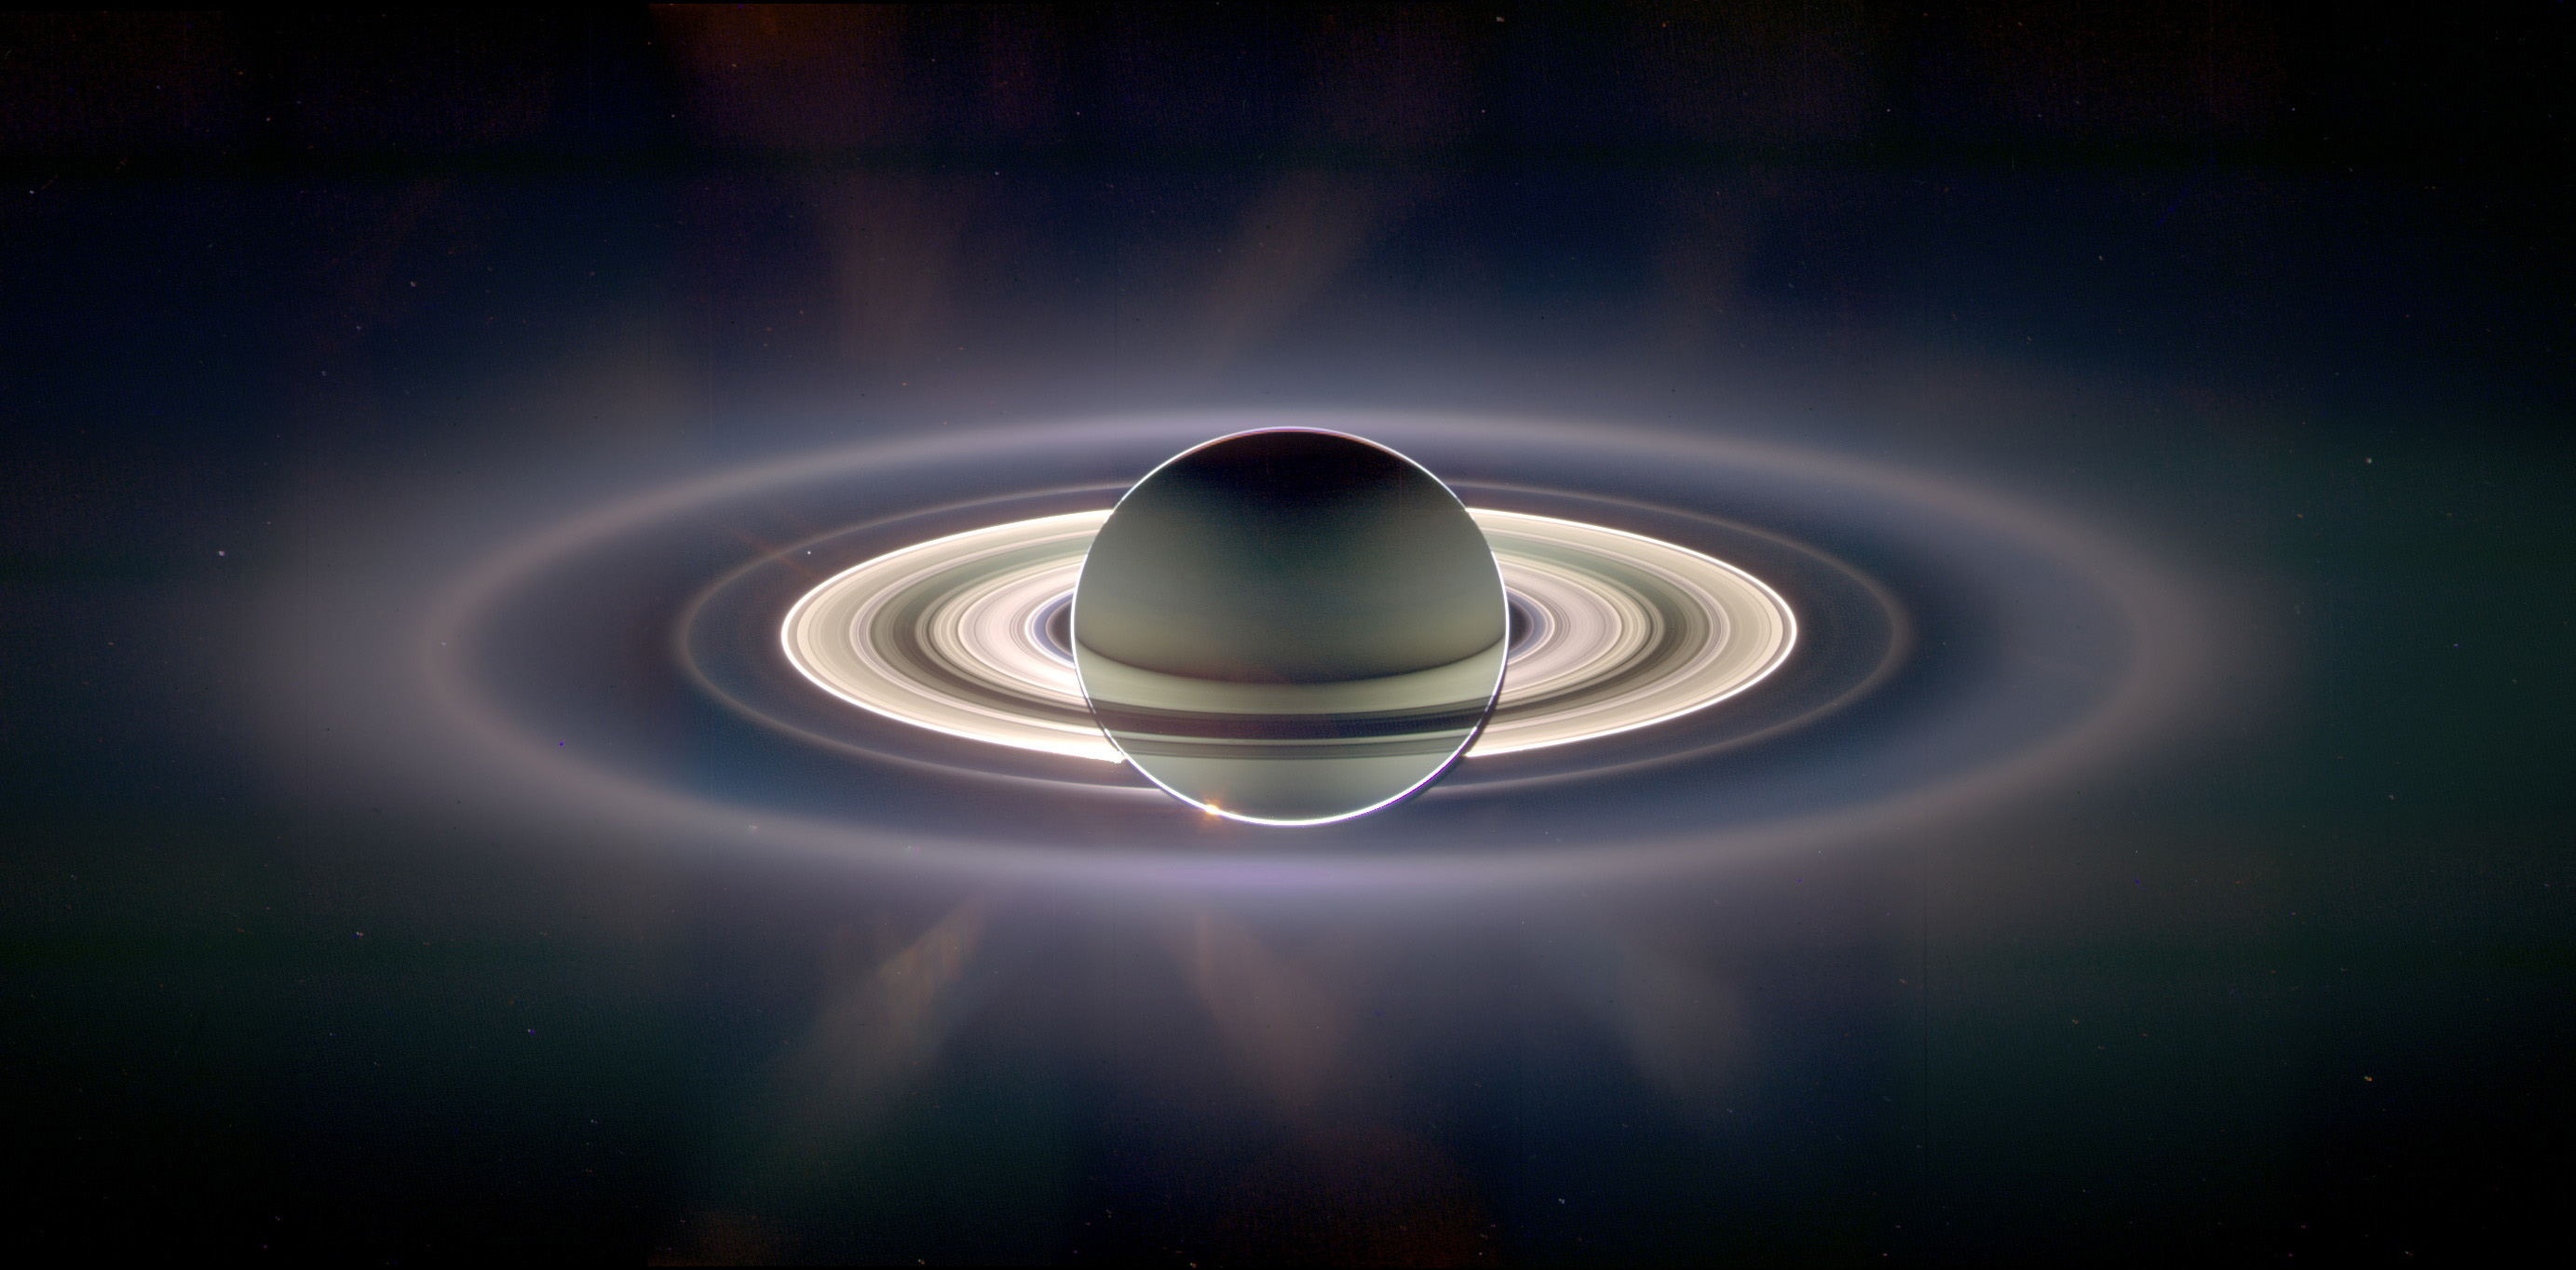
\includegraphics[width=\textwidth]{figures/newrings_cassini_big.jpg}
    \caption{Фотография Сатурна и его колец отправленная аппаратом Кассини в октябре 2009 года}
    \label{fig:cassini_saturn_panorama}
\end{figure}

Большая доля этих исследований посвящено изучению динамики и свойств колец Сатурна, которые являются ярким примером гранулярных газов в природе. 
Сами кольца состоят в основном из водяного льда и силикатных образований. Размеры частиц материала кольца составляют от микрометров до нескольких 
десятков метров. Объекты б\'{о}льших размеров, от нескольких сот метров до километров и более, классифицируются уже как отдельные луны Сатурна. 
Некоторые из подобных лун, как Пан и Дафнис (которые были обнаружены аппаратом Кассини), вращаются вокруг Сатурна на орбитах, находящихся внутри самих колец, 
имеют свое гравитационное поле которое серьезно воздействует на динамику мелких объектов кольца. Однако в нашей работе мы ограничимся системами, 
размеры составляющих частиц которых не превышают порядка нескольких метров. 
В этом случае можно исключить из рассмотрения гравитационные взаимодействия и сконцентрироваться только на контактных, механических
взаимодействиях при описании динамики гранулярного газа.

Для простоты описания механики столкновения частиц газа, будем рассматривать их как сферические объекты с заданными параметрами как
масса $m$, радиус $r$, модуль Юнга $Y$, коэффициент Пуассона $\eta$, поверхностная энергия (адгезивность) $\gamma$, коэффициент вязкой диссипации $A$.
Обозначенные выше параметры будут использованы для построения компьютерной модели столкновений, однако для теоретического описания системы
все механические свойства объединены в единый параметр, так называемый \emph{коэффициент реституции} -- $\eps$. Для описания динамики сухих
гранулярных газов, коэффициент реституции играет ключевую роль, и показывает количество диссипированной энергии при столкновениях. Математически
описывается следующим образом:
\begin{equation}\label{eq:restitution}
    \bg'_{12} = -\eps\bg_{12}\;,
\end{equation}
где $\bg_{12}$ -- относительная скорость частиц $1$ и $2$ \emph{до} столкновения, $\bg'_{12}$ -- относительная скорость \emph{после} столкновения.
Коэффициент реституции в общем случае всегда лежит в пределах $0\leq\eps\leq 1$. При $\eps = 0$ -- мы имеем абсолютно неупругое столкновение, 
при $\eps = 1$ -- абсолютно упругое столкновение. В данной работе мы будем рассматривать только сухие гранулярные системы, т. е. такие
системы для которых коэффициент адгезивности $\gamma = 0$. Таким образом, контактные взаимодействия частиц можно полностью описать двумя параметрами:
$r$ -- линейный размер частицы, который характеризует массу ($m\propto r^3$), поверхностное сечение ($\sigma\propto r^2$) и т.д., 
и $\eps$ -- коэффициент реституции, который описывает диссипативные свойства материала частицы. Мы будем предполагать, что материал частиц 
везде единообразен, и для всех столкновений $\eps$ будет одинаковый. 

Основным свойством гранулярного газа является его диссипативность, и как результат его \emph{гранулярная температура} имеет свойство всегда уменьшаться, 
т.е. предоставленный самому себе гранулярный газ, всегда будет \emph{охлаждаться}. Данное явление носит название закона Хаффа:
\begin{equation}
    T(t) = \frac{T_0}{(1+t/\tau_0)^2}\;, 
\end{equation}
где
\begin{equation}
    \tau^{-1}_0\propto n\sigma^2\left(1-\eps^2\right)\sqrt{T_0}\;.
\end{equation}
Таким образом, если в систему не подводить внешний источник энергии, то со временем гранулярный газ придет к состоянию с нулевой энергией. Здесь мы
коротко упомянули понятие гранулярной температуры, по аналогии с температурой обычных систем, однако оно не является температурой материала частицы 
в обычном понимании. Более детально мы рассмотрим ее в основной части работы.

Следующим важным моментом является \emph{полидисперсность} системы. До этого мы считали что все частицы в газе одинакового размера, однако в реальных
системах планетарных колец, размеры частиц очень сильно варьируются. Данное свойство привносит в систему один существенный эффект: если рассматривать
полидисперсную систему как смешение большого количества монодисперсных гранулярных газов с различными размерами, то парциальная температура каждого
из этих газов становится отличной друг от друга. Чем больше разница между размерами частиц этих монодисперсных газов, тем больше их разница в
гранулярной температуре. Конечно, без внешнего источника энергии, все эти температуры со временем сравняются и станут нулевыми. Однако планетарные
кольца находятся в центральном гравитационном поле своей планеты, и на самом деле являются дисками с дифференциальным вращением, и гранулярная система
подпитывается за счет гравитационной энергии своей планеты. Более подробно мы остановимся на данном явлении в основной части работы. Здесь же,
укажем что за счет данной подкачки энергии, температуры всех отдельных частей системы остановятся на определенном и различном стационарном значении, 
что является одним из результатов нашей работы. А также, мы покажем что подобная разница в стационарных температурах системы, оказывает влияние
на радиальное распределение размеров частиц друг относительно друга. Данный эффект неодинакового распределения частиц по размерам относительно
центрального поля хорошо виден на Рис.~\ref{fig:cassini_rings_radial_sizes}.

\begin{figure}[ht]
    \centering
    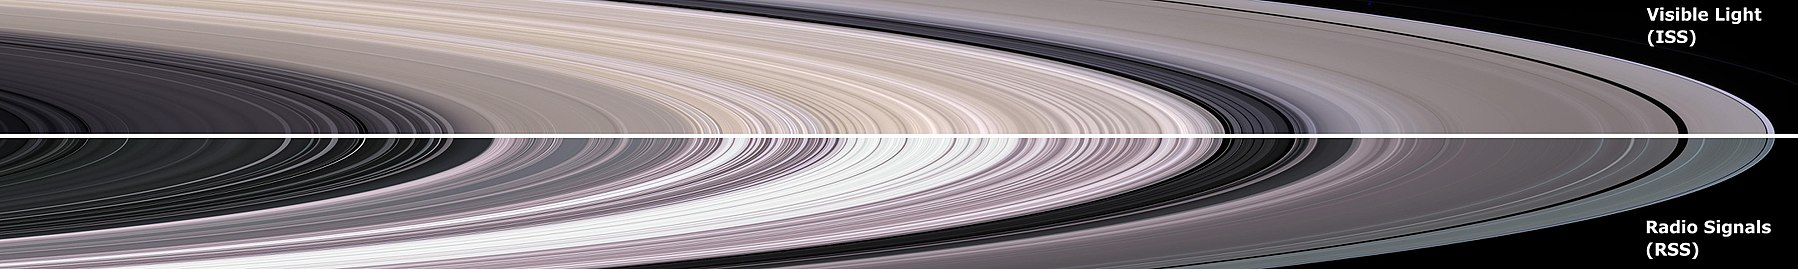
\includegraphics[width=\textwidth]{figures/1800px-Saturn's_rings_in_visible_light_and_radio.jpg}
    \caption{Фотография колец Сатурна в радиальном срезе. Верхняя часть показана в оптическом диапазоне, нижняя в радиоволновом диапазоне, 
    где цвета соотнесены с размерами частиц}
    \label{fig:cassini_rings_radial_sizes}
\end{figure}

\mainmatter % это включает нумерацию глав и секций в документе ниже

\chapter{Кинетическое описание полидисперсной системы}
\label{cha:analysis}

Для статистического описания неравновесной системы, мы будем исходить из кинетических уравнений Больцмана.
Перед этим нам необходимо определить фазовое пространство в котором происходит эволюция динамики отдельно
взятой частицы, а также более детально рассмотреть механику столкновений для составления интегралов столкновений.

\section{Уравнения Больцмана}

Рассмотрим весь газ как смесь из однородных газов, массы частиц в которых обозначим через $m$. Пусть $N_m$ будет 
количеством частиц массы $m$ в системе. Если общее количество частиц равно $N$, то
\begin{equation}
  \eta_m = \frac{N_m}{N}\;,
\end{equation}
относительное количество частиц массы $m$ в полной системе. Учитывая что количество частиц в планетарных кольцах огромно,
так же как и разновидность частиц по массе, то мы можем ввести функцию распределения особей в системе по массам как
\begin{equation}
  \eta(m) = \lim_{N\to\infty}\frac{N(m)}{N}\;,
\end{equation}
либо
\begin{equation}\label{eq:mass_distribution}
  \int\eta(m)\,dm=1\;.
\end{equation}
Здесь следует отметить, что как видно из \ref{eq:mass_distribution}, $\eta(m)\to 0$ при $m\to\infty$, что согласовывается 
с реальными наблюдениями. Таким образом, масса частицы $m$ будет показывать род подсистемы как непрерывная переменная.

Динамика отдельно взятой частицы массы $m$ описывается его векторами координат $\br$ и скоростей $\bv$ в фазовом пространстве.
В этом фазовом пространстве введем функцию распределения $f(t,m,\br,\bv)$ которое имеет следующее важное свойство:
\begin{equation}
  dN(t, m,\br,\bv) = f(t, m, \br, \bv)d\bv\;,
\end{equation}
где $dN(t, m, \br, \bv)$ -- функция числа частиц локализованных вокруг координаты $\br$ и имеющих скорости в диапазоне от
$\bv$ до $\bv+d\bv$. 
Так как газообразные системы являются разряженными, то макропараметры системы могут быть определены как
некие интегралы от одночастичной функции распределения. 

Нулевой момент дает нам функцию количественной плотности частиц
\begin{equation}
  n(t, m,\br) = \int f(t, m,\br,\bv)\,d\bv\;,
\end{equation}
либо функцию плотности масс
\begin{equation}
  \rho(t, m,\br) = mn(t, m,\br)=\int mf(t, m,\br,\bv)\,d\bv\;,
\end{equation}
и так далее. Более подробно макропараметры системы будут описаны при гидродинамическом описании системы.
Здесь же мы видим что параметры системы нестационарны и зависят от времени $t$, тогда как сама эволюция
функции распределения по времени подчиняется уравнению Больцмана \cite{Spahn:2004euro_lett_kinetic_fraggr,Dilley:1993icarus_energy_loss}:
\begin{equation}\label{eq:Boltzmann_general}
  \frac{\pd f}{\pd t} + \bv\frac{\pd f}{\pd\br} + \bw\frac{\pd f}{\pd v} = I_c(t,m,\br,\bv)\;,
\end{equation}
где $I_c(t,m,\br,\bv)$ -- полный интеграл столкновений, $\bw$ -- ускорение частицы под воздействием внешних сил.
Полный интеграл столкновений пишется через бинарный интеграл столкновений как:
\begin{equation}
  I_c(t,m,\br,\bv) = \int\eta(m')I_c(t,m',m,\br,\bv)\,dm'\;.
\end{equation}
Для нахождения точной формы интегралов столкновений необходимо более подробно изучить механику самих столкновений частиц.

\section{Механика столкновений}

Везде в дальнейшем мы будем предполагать, что все частицы в газе являются абсолютно сферическими и однородными,
с одинаковыми коэффициентами реституции $\eps$. При столкновении двух таких частиц, закон сохранения импульса запишется как:
\begin{equation}\label{eq:momentum_conservation}
  m_i\bv_i + m_j\bv_j = m_i\bv'_i+m_j\bv'_j\;,
\end{equation}
где знаками штриха $'$ обозначены скорости частиц после столкновения. Обмена массами и прилипания не происходит по условию задачи.
Для гранулярных газов закон сохранения энергии (механической) нарушается, а изменение относительных скоростей задается как:
\begin{equation}
  \bg'_{n} = -\eps\bg_{n}\;,
\end{equation}
где $\bg = \bg_{ij}=\bv_i-\bv_j$, а $\bg_n$ -- является нормальной составляющей относительной скорости. Определим нормальное 
направление столкновения как проходящей через центры сталкивающихся частиц в момент столкновения, и введем вектор
нормали:
\begin{equation}
  \bn = \bn_{ij} = \frac{\br_i-\br_j}{\sigma_i-\sigma_j}\;,
\end{equation}
где $\br_i,\;\br_j$ -- координаты частиц в момент столкновения.
Далее запишем изменение относительных скоростей следующим образом:
\begin{equation}
  (\bg'\cdot\bn)\bn = -\eps(\bg\cdot\bn)\bn\;,
\end{equation}
и подставляя в (\ref{eq:momentum_conservation}) получаем скорости частиц после столкновения:
\begin{equation}
  \begin{split}
    \bv'_i &= \bv_i - \frac{\mu}{m_i}(1+\eps)(\bg\cdot\bn)\bn\;,\\
    \bv'_j &= \bv_j + \frac{\mu}{m_j}(1+\eps)(\bg\cdot\bn)\bn\;,
  \end{split}  
\end{equation}
где $\mu=\mu_{ij}=\cfrac{m_im_j}{m_i+m_j}$ -- эффективная масса столкновения. Здесь следует иметь ввиду что вектор $\bn$
свободен и не зависит от значений скоростей.

Рассмотрим теперь изменение импульса частицы после столкновения:
\begin{equation}
  \delta\bm{p}_i = -\delta\bm{p}_j = \pm\mu(1+\eps)(\bg\cdot\bn)\bn\;.
\end{equation}
Знак переноса импульса зависит от взаимной конфигурации векторов $\bg$ и $\bn$, однако полное изменение импульса
конечно же $\delta\bm{p}_i+\delta\bm{p}_j=0$.

Теперь рассмотрим изменение кинетической энергии после столкновения:
\begin{equation}\label{eq:delta_E_v}
  \begin{split}
    \delta E_i &= \frac{m_i\bv^{'2}_i}{2}-\frac{m_i\bv^2_i}{2} 
    = -\mu(1+\eps)(\bg\cdot\bn)(\bv_i\cdot\bn)+\frac{\mu^2}{2m_i}(1+\eps)^2(\bg\cdot\bn)^2\;, \\
    \delta E_j &= \frac{m_j\bv^{'2}_j}{2}-\frac{m_j\bv^2_j}{2} 
    = +\mu(1+\eps)(\bg\cdot\bn)(\bv_j\cdot\bn)+\frac{\mu^2}{2m_j}(1+\eps)^2(\bg\cdot\bn)^2\;, \\
  \end{split}
\end{equation}
или перейдя в систему отсчета центра масс со скоростью $M\bv_C=m_i\bv_i+m_j\bv_j$, где $M=M_{ij}=m_i+m_j$, получим:
\begin{equation}
  \begin{split}
    \bv_i &= \bv_C + \frac{\mu}{m_i}\bg\;,\\
    \bv_j &= \bv_C - \frac{\mu}{m_j}\bg\;,
  \end{split}
\end{equation}
и соответственно
\begin{equation}\label{eq:delta_E}
  \begin{split}
    \delta E_i &= -\mu(1+\eps)(\bg\cdot\bn)(\bv_C\cdot\bn)-\frac{1-\eps^2}{2}\frac{\mu^2}{m_i}(\bg\cdot\bn)^2\;,\\
    \delta E_j &= +\mu(1+\eps)(\bg\cdot\bn)(\bv_C\cdot\bn)-\frac{1-\eps^2}{2}\frac{\mu^2}{m_j}(\bg\cdot\bn)^2\;.\\
  \end{split}
\end{equation}
Как видим, первые члены в правой части уравнений одинаковы и противоположны в знаках. Это означает что данная часть
кинетической энергии передается от одной частицы к другой, и остается в самой системе, не диссипируя. Вторые же
члены как мы видим всегда отрицательны и при разных массах $m_i\neq m_j$ также отличны друг от друга. Именно эта 
часть отвечает за диссипацию энергии в системе, и диссипация тем больше чем меньше коэффициент реституции $\eps$,
т.е. чем менее упругим будет столкновение, что вполне ожидаемо. Однако, как мы видим, диссипация также зависит
и от массы самой частицы, и чем \emph{меньше} масса частицы, тем \emph{больше} потери энергии:
\begin{equation}
  \left(\frac{\delta E_i}{\delta E_j}\right)_{diss}=\frac{m_j}{m_i}\;.
\end{equation}
Именно этот эффект приводит к нарушению равнораспределения энергии в полидисперсной системе гранулярных газов,
что в свою очередь приводит к неодинаковости гранулярных температур подсистем.
Полная потеря энергии при столкновении равна
\begin{equation}
  \delta E_i+\delta E_j = -\frac{1-\eps^2}{2}\mu(\bg\cdot\bn)^2\;.
\end{equation}

\section{Интеграл столкновений}
После описания механики столкновений, перейдем к самому виду интеграла столкновений в (\ref{eq:Boltzmann_general}).
В общем виде интеграл столкновений для гранулярных газов имеет вид:
\begin{equation}
  \begin{split}
    I_c(t,m_i,\br,\bv_i) &= \int dm_jg_2(\sigma_{ij})\eta(m_j)\sigma^{D-1}_{ij}\int d\bv_j\int d\bn\Theta(-\bg\cdot\bn)\vert\bg\cdot\bn\vert\times\\
    &\times\left(\frac{1}{\eps^2}f(t,m_i,\br,\bv''_i)f(t,m_j,\br,\bv''_j)-f(t,m_i,\br,\bv_i)f(t,m_j,\br,\bv_j)\right)\;,
  \end{split}
\end{equation}
где $\sigma_{ij}=\sigma_i+\sigma_j$ -- расстояние между центрами частиц, $g_2(\sigma_{ij})$ -- параметр Энскога, который учитывает
разницу в координатах центров частиц во время столкновений, который мы примем равным единице $g_2(\sigma_{ij})=1$, $\Theta(x)$ -- 
функция Хевисайда, которая включена для того чтобы учитывать только те соотношения скорости, при которых они сближаются, 
$\bv''_i,\;\bv''_j$ -- скорости обратных столкновений, $D$ -- размерность системы. По смыслу, интеграл столкновений показывает изменения 
в функции распределения за счет столкновений частиц. Интеграл столкновений имеет одно важное свойство, а именно, если взять некую 
динамическую функцию системы $\psi_i(\bv_i)$, и ее изменение после после прямого столкновения записать как 
$\Delta\psi_i(\bv_i)=\psi_i(\bv'_i)-\psi_i(\bv_i)$, то получим:
\begin{equation}\label{eq:collision_integral_dynamic_function}
  \begin{split}
    \frac{d}{dt}\langle\psi_i(\bv_i)\rangle_c &= \int\psi_i(\bv_i)\frac{\pd f_i}{\pd t}\,d\bv_i = \int\psi_i(\bv_i)I_c(t,m_i,\br,\bv_i)\,d\bv_i=\\
    &=\int dm_j\eta(m_j)\sigma^{D-1}_{ij}\int d\bv_id\bv_j\int d\bn\Theta(-\bg\cdot\bn)\vert\bg\cdot\bn\vert\times\\
    &\times f(t,m_i,\br,\bv_i)f(t,m_j,\br,\bv_j)\Delta\psi_i(\bv_i)\;.
  \end{split}
\end{equation}
Это свойство интеграла столкновения мы будем использовать в дальнейшем при описании эволюции энергии всей системы в целом.

\section{Эволюция энергии системы}
Для того чтобы оценить изменение энергии всей системы в целом за счет столкновений, возьмем функцию кинетической энергии
частицы как $\psi_i(\bv_i) = \cfrac{m_i\bv^2_i}{2}$, а вместо $\Delta\psi_i(\bv_i)=\delta E_i$ из уравнения (\ref{eq:delta_E}) и подставим
в (\ref{eq:collision_integral_dynamic_function}). В итоге получаем:
\begin{equation}\label{eq:energy_collision_evolution}
  \begin{split}
    \int\frac{m_iv^2_i}{2}I_c(t,m_i,\br,\bv_i)\,d\bv_i &= \int dm_j\eta(m_j)\sigma^{D-1}_{ij}
    \int d\bv_id\bg\int d\bn\Theta(-\bg\cdot\bn)\vert\bg\cdot\bn\vert\times\\
    &\times f(t,m_i,\br,\bv_i)f(t,m_j,\br,\bv_j)\delta E_i(\bv_i,\bg)\;,
  \end{split}
\end{equation}
здесь мы сделали замену переменных $d\bv_id\bv_j=d\bv_id\bg$. Для дальнейшего продвижения, нам необходимо знать вид самой функции распределения.


\chapter{Гидродинамическое описание системы}
\label{cha:design}

Перейдем теперь к более грубому, гидродинамическому описанию системы. Для начала нужно определить возможность такого перехода
в рассматриваемой нами системе. Через $L$ обозначим линейный размер всей системы в целом. Для кинетического описания нам было достаточно
что линейные размеры частиц $\sigma$ были намного меньше размера всей системы, т.е. выполнение условия $\sigma\ll L$. Соответственно
все кинетические уравнения пишутся на уровне детализации $\sigma$. Однако гидродинамическое описание происходит на другом уровне,
который мы обозначим $\ell$, и который удовлетворяет условию $\sigma\ll\ell\ll L$. Если мы можем вести изучение системы в таком масштабе,
то можно говорить что мы рассматриваем систему в гидродинамическом приближении. Линейные размеры колец Сатурна, т.е. ширина колец,
растягивается примерно на $L\sim 66 000$ км, в то время как размеры самих частиц варьируются в пределах $\sigma\sim 10^{-2}\div 10^2$ см.
Отсюда хорошо видно что можно подобрать такое значение $\ell\sim 1\div 2$ км, в пределах которого гидродинамическое описание системы
будет вполне оправдано. Таким образом, в дальнейшем мы можем говорить что в пределах $\ell$ вокруг координаты $\br$ находится достаточно большое
количество частиц, по которым можно определить макропараметры системы в зависимости от самой координаты $\br$. Перейдем к непосредственным 
определениям самих макропараметров, необходимых для полного гидродинамического описания системы, и написанию уравнений переноса
этих параметров.

\section{Уравнения переноса}

Зная функцию распределения, можно вводить пространственно распределенные параметры, описывающие систему в целом, а не через отдельно
взятые частицы. Такие параметры называются макропараметрами системы. Мы будем вводить их как моменты вектора скорости частиц $\bv$. Так,
нулевой момент, как мы уже ранее определили, дает нам функцию числовой плотности:
\begin{equation}
  n(t,m,\br) = \int f(t,m,\br,\bv)\,d\bv\;,
\end{equation}
либо функцию плотности масс
\begin{equation}\label{eq:mass_density}
  \rho(t,m,\br) = mn(t,m,\br) = \int mf(t,m,\br,\bv)\,d\bv\;.
\end{equation}
Данная функция читается так: $\rho(t,m,\br)$ -- это масса в единичном объеме участка кольца в координате $\br$ во время $t$, при этом 
масса вещества данного участка кольца равна $m$. Остальные параметры имеют схожий физический смысл.

Первый момент по скорости дает нам функцию плотности импульса
\begin{equation}\label{eq:momentum_density}
  \rho\bu(t,m,\br)=\int m\bv f(t,m,\br,\bv)\,d\bv\;,
\end{equation}
где $\bu$ -- дает нам среднюю скорость участка кольца. Введем понятие локальной скорости частиц
\begin{equation}\label{eq:local_velocity}
  \bc = \bv-\bu(t,m,\br)\;,
\end{equation}
которая показывает скорость (хаотического движения) частиц в системе отсчета движущейся вместе с участком кольца со скоростью $\bu$.
Таким образом введем понятие \emph{гранулярной температуры} системы, по аналогии с термодинамической температурой как второй момент
по скорости
\begin{equation}\label{eq:granular_temperature}
  \frac{D}{2}nT(t,m,\br) = \int\frac{m\bc^2}{2}f(t,m,\br,\bv)\,d\bv\;,
\end{equation}
где $D=3$ -- для трехмерной системы, однако мы будем рассматривать двумерную систему $D=2$.
Нам также понадобятся и другие моменты по скорости, которые уже являются тензорными величинами. Во первых, это
тензор \emph{напряжения}:
\begin{equation}
  \Pi_{\ab}(t,m,\br)=m\int v_\alpha v_\beta f(t,m,\br,\bv)\,d\bv\;,
\end{equation}
который можно разделить на две части используя (\ref{eq:local_velocity})
\begin{equation}
  \Pi_{\ab}(t,m,\br)=\rho u_\alpha u_\beta+P_{\ab}\;.
\end{equation}
Первая часть является динамической частью тензора напряжения, а вторая часть называется тензором \emph{внутренних напряжений}:
\begin{equation}
  P_{\ab}(t,m,\br)=m\int c_\alpha c_\beta f(t,m,\br,\bv)\,d\bv\;.
\end{equation}
Разделяя далее данный тензор на часть с нулевой сверткой и на диагональную часть, получаем:
\begin{equation}
  P_{\ab} = \delta_{\ab}p_{id}+\pi_{\ab}\;,\;\;\;\pi_{\alpha\alpha}=0\;,
\end{equation}
где 
\begin{equation}
  p_{id}=\frac{1}{D}\int m\bc^2f(t,m,\br,\bv)\,d\bv=nT\;,
\end{equation}
давление идеального газа. Часть тензора с нулевой сверткой $\pi_{\ab}$ также называется тензором \emph{вязких напряжений}.

Наконец, введем следующий тензор
\begin{equation}
  Q_{\ab\gamma}=m\int c_\alpha c_\beta c_\gamma f(t,m,\br,\bv)\,d\bv\;,
\end{equation}
или точнее его свертку по двум индексам
\begin{equation}
  q_\alpha=\bq = \frac{1}{2}Q_{\ab\beta} = \int \frac{m\bc^2}{2}c_\alpha f(t,m,\br,\bv)\,d\bv\;,
\end{equation}
который называется вектором \emph{потока тепла}.

Теперь приступим к написанию уравнений переноса для вышеперечисленных макропараметров. Для начала напишем
уравнение переноса для некоторой обобщенной динамической функции $A(t,m,\br,\bv)$. 
Умножим данную функцию на уравнение Больцмана (\ref{eq:Boltzmann_general})
и проинтегрируем по всему пространству скоростей:
\begin{equation}
  \int A\frac{\pd f}{\pd t}\,d\bv + \int A\bv\frac{\pd f}{\pd\br}\,d\bv+\int A\bw\frac{\pd f}{\pd\bv} 
  = \int AI_c(f,f')\,d\bv = \left\langle\frac{\pd A}{\pd t}\right\rangle_c\;,
\end{equation}
где правая часть показывает среднее изменение динамической функции по времени за счет столкновений.
Далее можно написать
\begin{equation}
  \int\left(\frac{\pd}{\pd t}(Af)+\frac{\pd}{\pd\br}(Af\bv)+\frac{\pd}{\pd\bv}(Af\bw)-
  f\left[\frac{\pd A}{\pd t}+\bv\frac{\pd A}{\pd\br}+\bw\frac{\pd A}{\pd\bv}\right]\right)
  \,d\bv=\left\langle\frac{\pd A}{\pd t}\right\rangle_c\;.
\end{equation}
Третий член в данном уравнении можно переписать используя теорему Гаусса
 \begin{equation}
   \int\frac{\pd}{\pd\bv}(Af\bw)\,d\bv=\oint Af\bw\cdot d\bm{\sigma} = 0\;.
 \end{equation}
Здесь, интегрирование по всему пространству скоростей заменено на интегрирование по контуру вокруг этого пространства, где
$v\to\pm\infty$. Однако функция распределения $f$ обращается в нуль в этом пределе по своей природе. Таким образом,
мы видим что этот интеграл исчезает. В конечном итоге у нас остается уравнение переноса в следующем виде:
\begin{equation}\label{eq:transport_equation_general}
  \frac{\pd}{\pd t}\int Af\,d\bv+\frac{\pd}{\pd\br}\int Af\bv\,d\bv
  -\int f\left[\frac{\pd A}{\pd t}+\bv\frac{\pd A}{\pd\bv}+\bw\frac{\pd A}{\pd\bv}\right]\,d\bv
  =\left\langle\frac{\pd A}{\pd t}\right\rangle_c\;.
\end{equation}
Теперь, подставляя вместо $A$ необходимые нам макропараметры системы, мы можем вывести соответствующие уравнения переноса для них.

\subsection{Перенос массы}
Заменяя в уравнении (\ref{eq:transport_equation_general}) динамическую функцию на массу, $A(t,m,\br,\bv)=m$, получаем
\begin{equation}
  \frac{\pd}{\pd t}\int mf\,d\bv + \frac{\pd}{\pd\br}\int mf\bv\,d\bv = 0\;,
\end{equation}
теперь используя (\ref{eq:mass_density}) и (\ref{eq:momentum_density}), получаем уравнение переноса плотности массы,
или так называемое \emph{уравнение непрерывности}
\begin{equation}
  \frac{\pd\rho}{\pd t}+\frac{\pd}{\pd\br}(\rho\bu)=0\;.
\end{equation}

\subsection{Перенос импульса}

Теперь вместо динамической функции подставляем импульс частицы 
$A(t,m,\br,\bv)=m\bv=mv_\alpha$, и получаем:
\begin{equation}
  \frac{\pd}{\pd t}\int m\bv f\,d\bv+\frac{\pd}{\pd r_\alpha}\int mfv_\alpha v_\beta\,d\bv-\bw\int mf\,d\bv = 
  \left\langle\frac{\pd(mv_{\alpha})}{\pd t}\right\rangle_c\;.
\end{equation}
Правая часть этого уравнения показывает изменение среднего импульса системы в целом, однако по закону сохранения импульса,
оно равняется нулю. Подставляя выражения соответствующих макропараметров, получаем:
\begin{equation}
  \frac{\pd(\rho\bu)}{\pd t} + \frac{\pd\Pi_{\ab}}{\pd r_\alpha} = \rho\bw\;,
\end{equation}
где правая часть $\rho\bw=\bm{F}_{ext}$ -- плотность внешних сил действующих на участок системы. В нашем случае
внешней силой является гравитационное воздействие планеты, которое записывается как $\bw=-\cfrac{\pd U(r)}{\pd\br}$,
где $r$ -- расстояние до центра планеты. Теперь разделяя тензор напряжений получаем уравнение переноса импульса
\begin{equation}
  \frac{\pd(\rho u_\alpha)}{\pd t} + \frac{\pd}{\pd r_\beta}(\rho u_\alpha u_\beta) = 
  -\frac{\pd\left(nT\right)}{\pd r_\alpha} - \frac{\pd\pi_{\ab}}{\pd r_\beta} + \rho w_\alpha\;.
\end{equation}

\subsection{Перенос энергии}

Теперь подставим функцию кинетической энергии $A(t,m,\br,\bv)=\cfrac{m\bv^2}{2}$ и запишем уравнение переноса
\begin{equation}
  \begin{split}
    &\frac{1}{2}\frac{\pd}{\pd t}\int m\left(\bc^2+2c_\alpha u_\alpha + \bu^2\right)f\,d\bv
    + \frac{1}{2}\frac{\pd}{\pd\br}\int m\left(\bc^2+2c_\alpha u_\alpha + \bu^2\right)v_\beta f\,d\bv-\\
    &-w_\beta\int mfv_\alpha\frac{\pd v_\alpha}{\pd v_\beta}\,d\bv=\left\langle\frac{\pd}{\pd t}\left(\frac{m\bv^2}{2}\right)\right\rangle_c=
    -T\xi(t,m,\br,T)\;.\\
  \end{split}
\end{equation}
По причине диссипативной природы гранулярных газов, закон сохранения энергии не выполняется, и соответственно правая часть уравнения показывает
среднее изменение энергии за счет столкновений. Здесь мы ввели положительную функцию $\xi(t,m,\br,T)$, которая отвечает за скорость
охлаждения газа. Точный вид этой функции мы выведем позднее. Продвигаясь далее записываем:
\begin{equation}
  \begin{split}
    &\frac{\pd}{\pd t}\int\frac{m\bc^2}{2}f\,d\bv+\frac{\pd}{\pd t}\int\frac{m\bu^2}{2}f\,d\bv+
    \frac{\pd}{\pd r_\beta}\int\frac{m\bc^2}{2}v_\beta f\,d\bv + \frac{\pd}{\pd r_\beta}\int\frac{m\bu^2}{2}v_\beta f\,d\bv + \\
    &+\frac{\pd}{\pd r_\beta}\int mc_\alpha u_\alpha v_\beta f\,d\bv = \delta_{\ab}w_\beta\rho u_\alpha - T\xi = u_\alpha\cdot\rho w_\alpha - T\xi\;,
  \end{split}
\end{equation}
где мы использовали условие $\int c_if\,d\bv=0$. Выражая через макропараметры, получаем:
\begin{equation}
  \begin{split}
    &\frac{\pd}{\pd t}\left(\frac{D}{2}nT+\frac{\rho\bu^2}{2}\right)+\frac{\pd}{\pd r_\beta}\int\frac{m\bc^2}{2}(c_\beta+u_\beta)\,d\bv +
    \frac{\pd}{\pd r_\beta}\int mfu_\alpha c_\alpha(c_\beta+u_\beta)\,d\bv +\\
    &+\frac{\pd}{\pd r_\beta}\left(\frac{\rho\bu^2}{2}u_\beta\right)=\rho\bw\cdot\bu-T\xi\;,
  \end{split}
\end{equation}
\begin{equation}
  \begin{split}
    &\frac{\pd}{\pd t}\left(\frac{D}{2}nT+\frac{\rho\bu^2}{2}\right)+\frac{\pd q_\alpha}{\pd r_\alpha}+
    \frac{\pd}{\pd r_\alpha}\left(\frac{D}{2}u_\alpha nT\right)+\frac{\pd}{\pd r_\alpha}u_\beta\int mfc_\alpha c_\beta\,d\bv+\\
    &+\frac{\pd}{\pd r_\alpha}\left(\frac{\rho\bu^2}{2}u_\alpha\right)=\rho\bw\cdot\bu-T\xi\;,
  \end{split}
\end{equation}
и используя выражение для тензора внутренних напряжений, получаем:
\begin{equation}
  \frac{\pd}{\pd t}\left(\frac{D}{2}nT+\frac{\rho\bu^2}{2}\right)+
  \frac{\pd}{\pd r_\alpha}\left(\frac{D}{2}u_\alpha nT+\frac{\rho\bu^2}{2}u_\alpha+\delta_{\ab}u_\beta nT+\pi_{\ab}u_\beta+q_\alpha\right)=
  \rho\bw\cdot\bu-T\xi\;,
\end{equation}
и в итоге получаем уравнение переноса энергии:
\begin{equation}
  \frac{\pd}{\pd t}\left(\frac{D}{2}nT+\frac{\rho\bu^2}{2}\right)+
  \frac{\pd}{\pd r_\alpha}u_\alpha\left(\frac{D+2}{2}nT+\frac{\rho\bu^2}{2}\right)+\frac{\pd}{\pd r_\alpha}(\pi_{\ab}u_\beta)
  +\frac{\pd q_\alpha}{\pd r_\alpha}=\rho\bw\cdot\bu-T\xi\;.
\end{equation}

\subsection{Вектор потока тепла и тензор вязких напряжений}

Во время вывода уравнений переноса, мы получили два неизвестных нам параметра, а именно $q_\alpha$ -- вектор потока тепла,
и $\pi_{\ab}$ -- тензор вязких напряжений. Выше, во время гидродинамического перехода, мы ввели некий размер в системе 
$\ell\ll L$. Если теперь рассмотреть малый параметр $x=\ell/L\ll 1$ вокруг которого разложим все макропараметры в ряд, то
в нулевом приближении оба параметра $q_\alpha$ и $\pi_{\ab}$ исчезают, так как в этом приближении мы имеем дело с идеальной
жидкостью. В линейном приближении по этому параметру, получаем $q_\alpha,\,\pi_{\ab}\sim x$, и они получают следующий вид
\begin{equation}\label{eq:viscosity_coeff}
  \begin{split}
    \pi_{\ab} &= -\nu\left(\frac{\pd u_\alpha}{\pd r_\beta}+\frac{\pd u_\beta}{\pd r_\alpha}
    -\frac{2}{D}\delta_{\ab}\frac{\pd u_\beta}{\pd r_\alpha}\right)\;,\\
    q_\alpha &= -\lambda\,\mbox{grad}\,T = -\lambda\frac{\pd T}{\pd r_\alpha}\;,
  \end{split}
\end{equation}
где $\nu$ -- коэффициент вязкости и $\lambda$ -- коэффициент теплопроводности.

\section{Скорость охлаждения системы}

Выше, при выводе уравнения переноса энергии, мы получили некую функцию $\xi(t,m,\br,T)$ которая показывает охлаждение
гранулярного газа за счет диссипативных столкновений. В общем виде эта функция определяется через интеграл столкновений,
как среднее изменение кинетической энергии:
\begin{equation}
  -T_i\xi(t,m_i,\br,T_i) = \int\frac{m_i\bv^2}{2}I_c(t,m_i,\br,\bv)\,d\bv\;.
\end{equation}
Здесь мы учли тот факт, что температуры отдельных подсистем могут быть отличны друг от друга, и показали эту зависимость
через индекс $i$. Используя свойство интеграла столкновений (\ref{eq:collision_integral_dynamic_function}), выпишем заново 
уравнение эволюции энергии системы за счет столкновений (\ref{eq:energy_collision_evolution})б в следующем виде:
\begin{equation}
  \begin{split}
    -T_i\xi(t,m_i,\br, T_i) &= 
    \int dm_j\eta(m_j)\sigma^{D-1}_{ij}\int d\bv_i d\bg\int d\bn\Theta(-\bg\cdot\bn)\vert\bg\cdot\bn\vert\times \\
    &\times f(t,m_i,\br,\bv_i)f(t,m_j,\br,\bv_i-\bg)\delta E_i(\bv_i,\bg) \;.
  \end{split}
\end{equation}

До сих пор мы ничего не говорили о виде самой функции распределения $f(t,m,\br,\bv)$, и все выводы получали для общего 
случая. Однако для дальнейшего продвижения нам необходимо указать вид этой функции. Функцию распределения можно представить
как разложение в ряд по малому параметру $x=\ell/L\ll 1$:
\begin{equation}
  f = f^{(0)} + c_1xf^{(1)}+c_2x^2f^{(2)}+\dots\;,
\end{equation}
где $c_i$ -- коэффициенты полина Сонина, $f^{(0)}$ -- нулевое приближение функции распределения, не что иное как функция
распределения Максвелла. Для простоты мы ограничимся этим приближением, так как его достаточно для описания исследуемых нами эффектов.
Таким образом, в дальнейшем принимаем:
\begin{equation}\label{eq:Maxwell_distribution}
  f(t,m_i,\br,\bv_i) = n_i \left(\frac{m_i}{2\pi T_i}\right)^{D/2}\cdot\exp\left\{-\frac{m_i\left(\bv_i-\bu_i\right)^2}{2T_i}\right\}\;,
\end{equation}
где $n_i$ -- числовая плотность частиц. Средняя скорость движения $\bu$ в нашем случае является скоростью на кеплеровской орбите, 
и зависит только от 
расстояния до центра планеты $\br$, и не зависит от массы частицы. Таким образом можно сделать замену переменных:
\begin{equation}
  \bc_i = \bv_i - \bu(\br)\;,\;\;\;d\bc_i=d\bv_i\;,
\end{equation}
и переписать функцию распределения в следующем виде:
\begin{equation}
  f(t,m_i,\br,\bc_i) = n_i\left(\frac{\kp_i}{\pi}\right)^{D/2}\cdot\exp\left(-\kp_ic^2_i\right)\;,
\end{equation}
где $\kp_i=\cfrac{m_i}{2T_i}$, и далее пишем:
\begin{equation}
  f(t,m_i,\br,\bc_i)f(t,m_j,\br,\bc_j)=n_in_j\left(\frac{\kp_i\kp_j}{\pi^2}\right)^{D/2}
  \cdot\exp\left(-\kp_ic^2_i-\kp_jc^2_j\right)\;.
\end{equation}
 Используя $\bv_i-\bv_j=\bc_i-\bc_j$ и соответственно $\bc_j=\bg-\bc_i$, перепишем выражение под экспонентой в следующем виде:
 \begin{equation}
   \begin{split}
     \kp_ic^2_i+\kp_jc^2_j &= \kp_ic^2_i+\kp_j(\bg-\bc_i)^2=\kp_ic^2_i+\kp_j\left(g^2+c^2_i-2\bg\cdot\bc_i\right)=\\
     &=(\kp_i+\kp_j)c^2_i+\kp_jg^2-2\kp_jgc_i\cos\gamma\;,
   \end{split}
 \end{equation}
где $\gamma$ -- угол между векторами $\bg$ и $\bc_i$. Теперь, среднее изменение некоторой динамической функции по времени
за счет столкновений можно представить с следующем виде:
\begin{equation}
  \begin{split}
    \frac{d}{dt}\langle\psi_i(\bc_i)\rangle &= \int dm_jn_in_j\eta(m_j)
    \sigma^{D-1}_{ij}\left(\frac{\kp_i\kp_j}{\pi^2}\right)^{D/2}\times\\
    &\times\int d\bc_id\bg\int d\bn\Theta(-\bg\cdot\bn)\vert\bg\cdot\bn\vert\times\\
    &\times\exp\left(-(\kp_i+\kp_j)c^2_i-\kp_jg^2+2\kp_jgc_i\cos\gamma\right)\Delta\psi_i(\bg,\bc_i)\;.
  \end{split}
\end{equation}


\subsection{Анализ диссипации для диска}
Для дальнейшего анализа, используем то обстоятельство, что кольца Сатурна являют чрезвычайно тонким и плоским образованием.
При радиальной ширине около $L\sim 66 000$ км, и азимутальной протяженности более полумиллиона километров, имеет толщину 
порядка нескольких метров. Данный факт делает кольцо Сатурна самым тонким природным образованием в солнечной системе. 
Нас же интересует радиальное распределение макропараметров, а не их распределение по толщине. Поэтому, во всех дальнейших
анализах примем рассматриваемую нами систему двумерной $D=2$. Полученные результаты будут отличаться от трехмерной системы
$D=3$ лишь некоторыми числовыми коэффициентами. Таким образом, интегрирование по сечению $d\bn\Theta(-\bg\cdot\bn)$ приводит
к интегралу по полуокружности, и дает нам $\pi$. Обозначая через $\theta$ угол между векторами $\bg$ и $\bn$, можно написать
$\vert\bg\cdot\bn\vert=g\cos\theta$, где $\theta$ меняется между $-\pi/2$ и $+\pi/2$. Перейдя в полярные координаты, получаем
$d\bc_id\bg=gc_i dg dc_id\theta d\gamma$, где $\gamma\in[0\div 2\pi]$. Подставляя все это в интеграл столкновений, пишем:
\begin{equation}
  \begin{split}
    \frac{d}{dt}\langle\psi_i(\bc_i)\rangle &=\frac{n_i\kp_i}{\pi}\int dm_jn_j\kp_j\eta(m_j)\sigma_{ij}
    \int dgdc_i\int_{-\pi/2}^{\pi/2}d\theta\int_0^{2\pi}d\gamma g^2c_i\cos\theta\times \\
    &\times\exp\left(-(\kp_i+\kp_j)c^2_i-\kp_jg^2+2\kp_jgc_i\cos\gamma\right)\Delta\psi_i(\bg,\bc_i)\;.
  \end{split}
\end{equation}
Теперь вместо $\psi_i(\bc_i)$ подставим (\ref{eq:delta_E_v}) и получаем:
\begin{equation}
  \begin{split}
    \left\langle\frac{dE_i}{dt}\right\rangle_c &= \frac{n_i\kp_i}{\pi}\int dm_jn_j\kp_j\eta(m_j)\sigma_{ij}
    \int dgdc_i g^2c_i\exp\left(-(\kp_i+\kp_j)c^2_i-\kp_jg^2\right)\times\\
    &\times\int_{-\pi/2}^{\pi/2}d\theta\cos\theta\int_{0}^{2\pi}d\gamma\exp(2\kp_jgc_i\cos\gamma)\times \\
    &\times\left(-\mu(1+\eps)gc_i\cos\theta\cos(\gamma-\theta)+\frac{\mu^2}{2m_i}(1+\eps)^2g^2\cos^2\theta\right)\;,
  \end{split}
\end{equation}
здесь мы использовали $\bc_i\cdot\bn=c_i\cos(\gamma-\theta)$. Рассмотрим отдельно угловые интегралы:
\begin{equation}
  \begin{split}
    S_{\theta\gamma,1} &= -\mu(1+\eps)gc_i\int_{-\pi/2}^{\pi/2}d\theta\cos^2\theta\int_{0}^{2\pi}d\gamma\cos(\theta-\gamma)\exp(R\cos\gamma)\;,\\
    S_{\theta\gamma,2} &= \frac{\mu^2g^2}{2m_i}(1+\eps)^2\int_{-\pi/2}^{\pi/2}d\theta\cos^3\theta\int_0^{2\pi}d\gamma\exp(R\cos\gamma)\;,
  \end{split}
\end{equation}
где $R=2\kp_jgc_i\geq 0$. Разложим первый интеграл по $\gamma$:
\begin{equation}
  \begin{split}
    S_{\gamma,1} &= \cos\theta\int_{0}^{2\pi}\cos\gamma\exp(R\cos\gamma)\,d\gamma+\sin\theta\int_{0}^{2\pi}\sin\gamma\exp(R\cos\gamma)\,d\gamma=\\
    &=\cos\theta\int_{0}^{2\pi}\cos\gamma\exp(R\cos\gamma)\,d\gamma = 2\cos\theta\int_{0}^{\pi}\cos\gamma\exp(R\cos\gamma)\,d\gamma\;.
  \end{split}
\end{equation}
Здесь функция под первым интегралом четная, поэтому ее можно разделить пополам, а функция под вторым интегралом нечетная, и поэтому исчезает.
Таким образом у нас остаются два интеграла по $\gamma$, которые не интегрируются в квадратурах, и представляются в виде модифицированных функций 
Бесселя:
\begin{equation}
  \begin{split}
    S_{\gamma,1} &= \int_{0}^{\pi}\cos\gamma\exp(R\cos\gamma)\,d\gamma = \pi I_1(R)\;,\\
    S_{\gamma,2} &= \int_{0}^{\pi}\exp(R\cos\gamma)\,d\gamma = \pi I_0(R)\;,
  \end{split}
\end{equation}
где
\begin{equation}
  I_\nu(x) = \frac{1}{\pi}\int_{0}^{\pi}e^{x\cos t}\cos(\nu t)\,dt-\frac{\sin(\pi\nu)}{\pi}\int_{0}^{\infty}e^{-x\cosh t-\nu t}\,dt\;,
\end{equation}
называется \emph{модифицированной функцией Бесселя}. Для значений параметра $\nu=0,\,1$ мы получаем наши интегралы по $\gamma$:
\begin{equation}
  \begin{split}
    S_{\theta\gamma,1} &= -\frac{8}{3}\pi\mu(1+\eps)gc_iI_1(R)\;,\\
    S_{\theta\gamma,2} &= \frac{4\pi\mu^2g^2}{3m_i}(1+\eps)^2I_0(R)\;,
  \end{split}
\end{equation}
где интеграл по $\theta$ элементарен:
\begin{equation}
  \begin{split}    
    \int_{-\pi/2}^{\pi/2} \cos^3\theta\,d\theta &= \frac{4}{3}\;.
  \end{split}
\end{equation}
Теперь исходный интеграл записывается в виде:
\begin{equation}
  \begin{split}
    \left\langle\frac{dE_i}{dt}\right\rangle_c &= \frac{4n_i\kp_i}{3}(1+\eps)\int dm_j\mu n_j\kp_j\eta(m_j)\sigma_{ij}
    \int dgdc_i g^3c_i\times\\
    &\times\exp(-(\kp_i+\kp_j)c^2_i-\kp_jg^2)\times\\
    &\times\left((1+\eps)\frac{\mu}{m_i}gI_0(R)-2c_iI_1(R)\right)\;,
  \end{split}
\end{equation}
или в более развернутом виде:
\begin{equation}
  \begin{split}
    \left\langle\frac{dE_i}{dt}\right\rangle_c &= \frac{4n_i\kp_i}{3}(1+\eps)\int dm_j\mu n_j\kp_j\eta(m_j)\sigma_{ij}
    \int_{0}^{\infty}dg\,g^3e^{-\kp_jg^2}\times\\
    &\times\int_{0}^{\infty}dc_i\,c_i\exp\left(-(\kp_i+\kp_j)c^2_i\right)\times\\
    &\times\left\{(1+\eps)\frac{\mu}{m_i}gI_0(2\kp_jgc_i)-2c_iI_1(2\kp_jgc_i)\right\}\;.
  \end{split}
\end{equation}
Интегралы по функциям Бесселя могут быть рассчитаны с помощью следующих формул:
\begin{equation}
  \begin{split}
    \int_{0}^{\infty}&x^{\alpha-1}e^{-px^2}I_{\nu}(cx)\,dx = A^{\alpha}_{\nu}\;,\;\;\;\left[\Re(p),\;\Re(\alpha+\nu)>0,\;\vert\arg c\vert<\pi\right]\;,\\
    &A^{\alpha}_{\nu}=2^{-\nu-1}c^{\nu}p^{-(\alpha+\nu)/2}\cdot\frac{\Gamma((\alpha+\nu)/2)}{\Gamma(\nu+1)}\cdot
    \mbox{}_{1}F_{1}\left(\frac{\alpha+\nu}{2};\;\nu+1;\;\frac{c^2}{4p}\right)\;,
  \end{split}
\end{equation}
где 
\begin{equation}
  \mbox{}_{1}F_{1}(a;\,b;\,z) = \sum_{n=0}^{\infty}\frac{a^{(a)}z^n}{b^{(n)}n!}\;,
\end{equation}
называется \emph{вырожденной гипергеометрической функцией}. Для наших интегралов, нам нужны два специальных случая:
\begin{equation}
  \begin{split}
    \int_{0}^{\infty}xe^{-px^2}I_0(cx)\,dx &= A^{2}_{0}\;,\\
    \int_{0}^{\infty}x^2e^{-px^2}I_1(cx)\,dx &= A^{3}_{1}\;,
  \end{split}
\end{equation}
где
\begin{equation}
  \begin{split}
    p &= \kp_i+\kp_j\;,\\
    c &= 2\kp_jg\;.
  \end{split}
\end{equation}
Если выполняется условие $\alpha=\nu+2$, то интегральная формула может быть сильно упрощена:
\begin{equation}
  A^{\nu+2}_{\nu} = \frac{c^{\nu}}{(2p)^{\nu+1}}\exp\left(\frac{c^2}{4p}\right)\;.
\end{equation}
В итоге получаем:
\begin{equation}
  \begin{split}
    \int_{0}^{\infty}xe^{-px^2}I_0(cx)\,dx &= \frac{1}{2p}\exp\left(\frac{c^2}{4p}\right)\;,\\
    \int_{0}^{\infty}x^2e^{-px^2}I_1(cx)\,dx &= \frac{c}{(2p)^2}\exp\left(\frac{c^2}{4p}\right)\;.
  \end{split}
\end{equation}
Подставляя все выражения на места, и имея ввиду табличный интеграл:
\begin{equation}      
    \int_{0}^{\infty}x^4e^{-ax^2}\,dx = \frac{3}{8a^2}\sqrt{\frac{\pi}{a}}\;,
\end{equation}
получаем:
\begin{equation}  
    \left\langle\frac{dE_i}{dt}\right\rangle_c = \frac{\sqrt{\pi}}{2}\int dm_j\Lambda_{ij}\mu(1+\eps)
    \frac{\kp_i+\kp_j}{\kp_i\kp_j}\sqrt{\frac{\kp_i+\kp_j}{\kp_i\kp_j}}\left(\frac{1+\eps}{2}\frac{\mu}{m_i}
    -\frac{\kp_j}{\kp_i+\kp_j}\right)\;,
\end{equation}
где
\begin{equation}
  \Lambda_{ij} = n_in_j\eta(m_j)\sigma_{ij}\;.
\end{equation}
Обозначая $\eta(m_j)dm_j=d\chi_j$ -- количество частиц подсистемы $j$ в элементарном объеме вокруг $\br$, получаем
\begin{equation}  
    \left\langle\frac{dE_i}{dt}\right\rangle_c = \frac{\sqrt{\pi}}{2}\cdot n_i(1+\eps)\int d\chi_jn_j \sigma_{ij}\mu_{ij}
    \frac{\kp_i+\kp_j}{\kp_i\kp_j}\sqrt{\frac{\kp_i+\kp_j}{\kp_i\kp_j}}\left(\frac{1+\eps}{2}\frac{\mu_{ij}}{m_i}
    -\frac{\kp_j}{\kp_i+\kp_j}\right)\;,    
\end{equation}
Продвигаемся далее. Так как:
\begin{equation}
  \frac{\kp_j}{\kp_i+\kp_j} = \frac{m_jT_i}{m_iT_j+m_jT_i}\;,
\end{equation}
и
\begin{equation}
  \mu_{ij}\cdot\frac{\kp_i+\kp_j}{\kp_i\kp_j} = \frac{m_im_j}{m_i+m_j}\frac{\frac{m_i}{2T_i}+\frac{m_j}{2T_j}}{\frac{m_im_j}{4T_iT_j}}=
  2\cdot\frac{m_iT_j+m_jT_i}{m_i+m_j}\;,
\end{equation}
преобразуем выражение под интегралом
\begin{equation*}
  \begin{split}
    S &= \mu_{ij}(1+\eps)\frac{\kp_i+\kp_j}{\kp_i\kp_j}\times\left(\frac{\mu_{ij}(1+\eps)}{2m_i}-\frac{\kp_j}{\kp_i+\kp_j}\right) = \\
    &= \frac{m_iT_j+m_jT_i}{m_i+m_j}\left(\frac{m_j}{m_i+m_j}(1+\eps)^2-\frac{2(1+\eps)m_jT_i}{m_iT_j+m_jT_i}\right)=\\
    &= \frac{m_j}{(m_i+m_j)^2}\left((m_iT_j+m_jT_i)(1+\eps)^2-2(1+\eps)(m_i+m_j)T_i\right)=\\
    &= \frac{m_j}{(m_i+m_j)^2}\left([(1+\eps)^2T_j-2(1+\eps)T_i]m_i+[(1+\eps)^2-2(1+\eps)]m_jT_i\right)=\\
    &= \frac{m_j}{(m_i+m_j)^2}\left(-\left(1-\eps^2\right)m_jT_i+(1+\eps)[(1+\eps)T_j-2T_i]m_i\right)\;,
  \end{split}
\end{equation*}
далее, имея ввиду что $2=1+\eps+1-\eps$, пишем:
\begin{equation*}
  \begin{split}
    S &= \frac{m_j}{(m_i+m_j)^2}\left(-\left(1-\eps^2\right)m_jT_i+m_i(1+\eps)[(1+\eps)T_j-(1+\eps)T_i-(1-\eps)T_i]\right)=\\
    &= \frac{m_j}{(m_i+m_j)^2}\left(-\left(1-\eps^2\right)m_jT_i+m_i(1+\eps)^2\left(T_j-T_i\right)-m_i\left(1-\eps^2\right)T_i\right) =\\
    &= \frac{m_j}{(m_i+m_j)^2}\left(-\left(1-\eps^2\right)(m_i+m_j)T_i+m_i(1+\eps)^2\left(T_j-T_i\right)\right)=\\
    &= -\left(1-\eps^2\right)\frac{m_j}{m_i+m_j}T_i+(1+\eps)^2\frac{m_im_j}{(m_i+m_j)^2}\left(T_j-T_i\right)\;,
  \end{split}
\end{equation*}
и наконец
\begin{equation}
  S = -\left(1-\eps^2\right)\frac{\mu}{m_i}T_i+(1+\eps)^2\frac{\mu^2}{m_im_j}\left(T_j-T_i\right)\;.
\end{equation}
Вставляя полученное выражение в исходный интеграл, получаем:
\begin{equation}\label{eq:cooling_rate_interm}
  \begin{split}
    \left\langle\frac{dE_i}{dt}\right\rangle_c &= \sqrt{\frac{\pi}{2}}\cdot n_i\int d\chi_jn_j\sigma_{ij}
    \sqrt{\frac{m_iT_j+m_jT_i}{m_im_j}}\times \\
    &\times\left(-\left(1-\eps^2\right)\frac{\mu}{m_i}T_i+(1+\eps)^2\frac{\mu^2}{m_im_j}(T_j-T_i)\right)\;.    
  \end{split}
\end{equation}

\subsection{Усредненные по ансамблю динамические параметры смеси гранулярных газов}
Рассмотрим некоторые динамические параметры смеси гранулярных газов, которые будут необходимы нам для дальнейшего анализа.
Возьмем некоторую функцию зависящую от двухчастичного распределения $\alpha_{ij}$. В общем виде, среднее значение
двухчастичной функции задается следующим выражением:
\begin{equation}
  \begin{split}
    \langle \alpha_{ij}\rangle &= \frac{\int \alpha_{ij}\cdot f(t,m_i,\br,\bc_i)f(t,m_j,\br,\bc_j)\,d\bc_id\bc_j}
    {\int f(t,m_i,\br,\bc_i)f(t,m_j,\br,\bc_j)\,d\bc_id\bc_j} = \\
    &= \frac{1}{n_in_j}\int \alpha_{ij}\cdot f(t,m_i,\br,\bc_i)f(t,m_j,\br,\bc_j)\,d\bc_id\bc_j\;,
  \end{split}
\end{equation}
и принимая во внимание что функцию распределения мы выбрали в виде Максвелловского распределения (\ref{eq:Maxwell_distribution}), и 
следуя такой же схеме рассуждений как и в предыдущей главе, пишем:
\begin{equation}
  \begin{split}
    \langle \alpha_{ij}\rangle &= \frac{\kp_i\kp_j}{\pi^2}\int_{0}^{\infty}dg\,ge^{-\kp_jg^2}\int_{0}^{\infty}dc_i\,c_i\alpha_{ij}e^{-(\kp_i+\kp_j)c^2_i}
    \int_{0}^{2\pi}d\phi\int_{0}^{2\pi}d\gamma\,\exp(2\kp_jgc_i\cos\gamma)=\\
    &=4\kp_i\kp_j\int_{0}^{\infty}dg\,ge^{-\kp_jg^2}\int_{0}^{\infty}dc_i\,c_i\alpha_{ij}I_0(2\kp_jg\cdot c_i)
    \exp\left(-(\kp_i+\kp_j)c^2_i\right)\;,
  \end{split}
\end{equation}
где под $\alpha_{ij}$ мы понимаем некоторую функцию по комбинациям скоростей частиц. Сначала положим $\alpha_{ij}=g_{ij}$, 
и в итоге получаем среднюю скорость столкновений для частиц подсистем $i$ и $j$ для двумерного газа:
\begin{equation}
    \langle g_{ij}\rangle = 4\kp_i\kp_j\int_{0}^{\infty}dg\,g^2e^{-\kp_jg^2}\int_{0}^{\infty}dc_i\,c_i
    I_0(\lambda\cdot c_i)\exp\left(-pc^2_i\right)\;,
\end{equation}
где $p=\kp_i+\kp_j$, $\lambda = 2\kp_j g$. Нам также понадобятся и другие динамические параметры. Это среднее по ансамблю
квадрата скорости столкновения, которое присутствует в выражениях для энергии в системе.
\begin{equation}
  \langle g^2_{ij}\rangle = 4\kp_i\kp_j\int_{0}^{\infty}dg\,g^3e^{-\kp_jg^2}\int_{0}^{\infty}dc_i\,c_i
  I_0(\lambda\cdot c_i)\exp\left(-pc^2_i\right)\;.
\end{equation}
Также запишем следующую функцию $\alpha_{ij} = \bg_{ij}\cdot\bc_i=g_{ij}c_i\cos\gamma$, и получаем:
\begin{equation}
  \langle \bg_{ij}\cdot\bc_i\rangle = 4\kp_i\kp_j\int_{0}^{\infty}dg\,g^2e^{-\kp_jg^2}\int_{0}^{\infty}dc_i\,c^2_i
  I_1(\lambda\cdot c_i)\exp\left(-pc^2_i\right)\;.
\end{equation}
Таким образом:
\begin{equation}
  \begin{split}
    \langle g_{ij}\rangle &= 4\kp_i\kp_j\int_{0}^{\infty}dg\,g^2e^{-\kp_jg^2}\cdot\frac{1}{2p}\exp\left(\frac{\lambda^2}{4p}\right)\;,\\
    \langle g^2_{ij}\rangle &= 4\kp_i\kp_j\int_{0}^{\infty}dg\,g^3e^{-\kp_jg^2}\cdot\frac{1}{2p}\exp\left(\frac{\lambda^2}{4p}\right)\;,\\
    \langle \bg_{ij}\cdot\bc_i\rangle &= 4\kp_i\kp_j\int_{0}^{\infty}dg\,g^2e^{-\kp_jg^2}\cdot\frac{\lambda}{4p^2}\exp\left(\frac{\lambda^2}{4p}\right)\;,
  \end{split}
\end{equation}
или
\begin{equation}
  \begin{split}
    \langle g_{ij}\rangle &= 2R\int_{0}^{\infty}dg\,g^2e^{-Rg^2}=\frac{1}{2}\sqrt{\frac{\pi}{R}}\;,\\
    \langle g^2_{ij}\rangle &= 2R\int_{0}^{\infty}dg\,g^3e^{-Rg^2}=\frac{1}{R}\;,\\
    \langle \bg_{ij}\cdot\bc_i\rangle &= \frac{2R^2}{\kp_i}\int_{0}^{\infty}dg\,g^3e^{-Rg^2}=\frac{1}{\kp_i}\;,
  \end{split}
\end{equation}
где 
\begin{equation}
  R=\frac{\kp_i\kp_j}{\kp_i+\kp_j}=\frac{1}{2}\frac{m_im_j}{m_iT_j+m_jT_i}\;.
\end{equation}
В конечном итоге получаем:
\begin{equation}
  \begin{split}
    \langle g_{ij}\rangle &= \sqrt{\frac{\pi}{2}}\cdot\sqrt{\frac{m_iT_j+m_jT_i}{m_im_j}}\;,\\
    \langle g^2_{ij}\rangle &= 2\cdot\frac{m_iT_j+m_jT_i}{m_im_j}\;,\\
    \langle \bg_{ij}\cdot\bc_i\rangle &= \frac{2T_i}{m_i}\;.
  \end{split}
\end{equation}

Оценим частоту столкновений частицы подсистемы $i$ с частицами подсистемы $j$. Представим что размер частицы $i$ пренебрежимо
мал, и она движется среди других частиц с размерами $\sigma_{ij}=\sigma_i+\sigma_j$, и плотностью $n_j$. В таком случае частота
столкновений равна:
\begin{equation}
  \omega_{ij} = \sigma_{ij}n_j\langle g_{ij}\rangle=\sqrt{\frac{\pi}{2}}\cdot\sigma_{ij}n_j\sqrt{\frac{m_iT_j+m_jT_i}{m_im_j}}\;.
\end{equation}
Теперь посчитаем среднее по ансамблю изменение энергии при столкновениях
(\ref{eq:delta_E}):
\begin{equation}
  \begin{split}
    \langle\delta E_i\rangle &= -\mu(1+\eps)\langle \bg\cdot\bv_C\rangle-\frac{1-\eps^2}{2}\frac{\mu^2}{m_i}\langle g^2\rangle=\\
    &=-\frac{\mu^2}{m_j}(1+\eps)\langle \bg\cdot\bc_i\rangle-\frac{\mu^2}{m_i}(1+\eps)\langle \bg\cdot\bc_j\rangle
    -\frac{1-\eps^2}{2}\frac{\mu^2}{m_i}\langle g^2\rangle = \\
    &=-\frac{\mu^2}{m_j}(1+\eps)\langle \bg\cdot\bc_i\rangle-\frac{\mu^2}{m_i}(1+\eps)\langle \bg\cdot(\bc_i-\bg)\rangle
    -\frac{1-\eps^2}{2}\frac{\mu^2}{m_i}\langle g^2\rangle = \\
    &=-\mu(1+\eps)\langle \bg\cdot\bc_i\rangle+\frac{\mu^2}{m_i}(1+\eps)\langle g^2\rangle
    -\frac{1-\eps^2}{2}\frac{\mu^2}{m_i}\langle g^2\rangle = \\
    &=-\mu(1+\eps)\langle \bg\cdot\bc_i\rangle+\frac{\mu^2}{m_i}\frac{(1+\eps)^2}{2}\langle g^2\rangle \;,
  \end{split}
\end{equation}
далее пишем:
\begin{equation}
  \begin{split}
    \langle\delta E_i\rangle &=-\mu(1+\eps)\frac{2T_i}{m_i}+\frac{\mu^2}{m_i}(1+\eps)^2\cdot\frac{m_iT_j+m_jT_i}{m_im_j}=\\
    &=\frac{\mu}{m_i}(1+\eps)\left((1+\eps)\cdot\frac{m_iT_j+m_jT_i}{m_i+m_j}-2T_i\right)=\\
    &=\frac{\mu}{m_i}\frac{1+\eps}{m_i+m_j}\left[(1+\eps)m_iT_j+(1+\eps)m_jT_i-2m_iT_i-2m_jT_i\right]=\\
    &=\frac{\mu}{m_i}\frac{1+\eps}{m_i+m_j}\left[(1+\eps)m_i(T_j-T_i)-(1-\eps)(m_i+m_j)T_i\right]\;,
  \end{split}
\end{equation}
и в итоге получаем:
\begin{equation}
  \langle\delta E_i\rangle = -\left(1-\eps^2\right)\frac{\mu}{m_i}T_i+(1+\eps)^2\frac{\mu^2}{m_im_j}(T_j-T_i)\;.
\end{equation}
Данное выражение равно выражению под скобкой в уравнении (\ref{eq:cooling_rate_interm}), и в итоге ее можно переписать в
следующем виде:
\begin{equation}
  \left\langle\frac{dE_i}{dt}\right\rangle_c = n_i\int d\chi_j\omega_{ij}\langle\delta E_i\rangle\;.
\end{equation} 
Вспомним что скорость изменения энергии системы за счет столкновений мы выразили через функцию охлаждения $\xi(t,m_i,\br,T_i)$, 
и теперь мы можем написать вид этой функции следующим образом:
\begin{equation}
  \left\langle\frac{dE_i}{dt}\right\rangle_c = -T_i\xi(t,m_i,\br,T_i)\;,
\end{equation} 
или
\begin{equation}\label{eq:cooling_term}
  \xi(t,m_i,\br,T_i)=-\frac{n_i}{T_i}\int d\chi_i\omega_{ij}\left(-A_{ij}T_i+B_{ij}(T_j-T_i)\right)\;,
\end{equation}
где
\begin{equation}
  \begin{split}
    A_{ij} &= \left(1-\eps^2\right)\frac{\mu}{m_i}\;,\\
    B_{ij} &= (1+\eps)^2\frac{\mu^2}{m_im_j}\;.
  \end{split}
\end{equation}
Здесь, параметр $A_{ij}$ показывает скорость охлаждения системы из-за диссипации при столкновениях, 
параметр $B_{ij}$ показывает скорость обмена энергии между подсистемами $i$ и $j$. Данная часть энергии
остается в системе, и не диссипирует.

\subsection{Нормальное решение и приближение по среднему полю}
Рассматриваемая нами система полидисперсных гранулярных газов, после начального релаксационного периода, приходит 
к универсальному, т.н. \emph{нормальному} решению. Смысл этого решения в том, что все зависимости функции
распределения от времени и пространства выражаются только через гидродинамические (макроскопические) параметры системы, 
такие как плотность числа, гранулярная температура, средняя скорость потока и т.д. Самой важной особенностью данного решения
в том, что все подсистемы охлаждаются с одинаковой скоростью. Отсюда мы понимаем, что неодинаковость температур подсистем,
появляется в начальной стадии эволюции системы, затем можно предположить что они эволюционируют независимо друг от друга,
с различными начальными температурами, до тех пор пока системы не приходит к стационарному состоянию, при котором диссипация
компенсируется подкачкой энергии в систему, и все подсистемы приходят к своим собственным стационарным температурам.
Одинаковость скорости охлаждения выражается следующим образом:
\begin{equation}
  \frac{1}{T_i}\frac{dT_i}{dt}=\frac{1}{T_j}\frac{dT_j}{dt}=-\xi(t)\;.
\end{equation}

Используя нормальное решение системы, введем понятие \emph{среднего поля}. Это некая мнимая подсистема, с некоторой массой 
мнимых частиц $\bar{m}$, и некоторой мнимой температурой $\bar{T}$. Эти величины характеризуются полидисперсностью системы в целом
и имеют следующий вид:
\begin{equation}
  \begin{split}
    \bar{T} &= \int d\chi_iT_i\;,\\
    \bar{m} &= \int d\chi_im_i\;.
  \end{split}
\end{equation}
Теперь возьмем уравнение для охлаждения системы (\ref{eq:cooling_term}), и проинтегрируем по всему ансамблю:
\begin{equation}
  \begin{split}
    \frac{d}{dt}\int d\chi_iT_i &= -\int d\chi_iT_i\xi_i(t) = -\int d\chi_i\int d\chi_j\omega_{ij}(A_{ij}T_i-B_{ij}(T_j-T_i))=\\
    &=-\int d\chi_iT_i\int d\chi_j\omega_{ij}A_{ij}+\iint d\chi_id\chi_j\omega_{ij}B_{ij}(T_j-T_i)\;.
  \end{split}
\end{equation}
Так как параметр $B_{ij}$ отвечает за перенос энергии внутри системы, и не участвует в диссипации, то при интегрировании по
всей системе, последний интеграл исчезает, это также видно по тому факту, что выражение под интегралом является антисимметричным.
Таким образом, получаем:
\begin{equation}\label{eq:mean_field_temp_interm}
  \frac{d\bar{T}}{dt}=-\int d\chi_iT_i\int d\chi_j\omega_{ij}A_{ij}\;.
\end{equation}
С другой стороны, для нормального решения, мы также можем написать:
\begin{equation}
  \frac{dT_i}{dt}=-\xi(t)T_i\;,
\end{equation}
и интегрируя по всему ансамблю получаем:
\begin{equation}
  \int d\chi_i\frac{dT_i}{dt}=-\int d\chi_i\xi(t)T_i\;,
\end{equation}
или
\begin{equation}
  \frac{d\bar{T}}{dt}=-\xi(t)\bar{T}\;.
\end{equation}
Приравнивая к (\ref{eq:mean_field_temp_interm}), получаем:
\begin{equation}
  \xi(t) = \frac{\int d\chi_iT_i\int d\chi_j\omega_{ij}A_{ij}}{\int d\chi_iT_i}\;.
\end{equation}
Для дальнейшего продвижения, сделаем т.н. \emph{аппроксимацию по среднему полю}. Предположим, что всю систему 
можно заменить монодисперсной системой с макропараметрами, поведение которых такое же как и у изначальной системы.
В таком случае, напишем:
\begin{equation}
  \xi(t)\approx\frac{\bar{T}\cdot\int d\chi_i\omega_{ij}A_{ij}}{\bar{T}}=\bar{\omega}\bar{A}\;,
\end{equation}
где $\bar{\omega}$ -- средняя частота столкновений. Для колец Сатурна нам известно, что 
\begin{equation}
  \bar{\omega}\approx3\Omega\tau\;,
\end{equation}
где $\tau$ -- оптическая толщина кольца. Диссипативный параметр $\bar{A}$ имеет форму:
\begin{equation}
  \bar{A}\propto\frac{1-\eps^2}{2}\;,
\end{equation}
и в итоге можно написать:
\begin{equation}
  \xi(t)=\xi\approx\frac{3}{2}\left(1-\eps^2\right)\Omega\tau\;.
\end{equation}
\chapter{Диск с дифференциальным вращением}
\label{cha:impl}

 Мы вывели гидродинамические уравнения переноса и скорость охлаждения системы за счет столкновений.
 Выпишем эти уравнения заново:
 \begin{equation}
    \begin{split}
        \frac{\pd\rho}{\pd t}+\frac{\pd}{\pd r_{\alpha}}(\rho u_{\alpha}) &=0\;\\
        \frac{\pd(\rho u_{\alpha})}{\pd t} + \frac{\pd}{\pd r_{\beta}}(\rho u_{\alpha}u_{\beta}) 
        &= -\frac{\pd (nT)}{\pd r_{\alpha}}-\frac{\pd\pi_{\ab}}{\pd r_{\beta}}+\rho w_{\alpha}\;,\\
        \frac{\pd}{\pd t}\left(nT+\frac{\rho u_{\beta}u_{\beta}}{2}\right) + \frac{\pd}{\pd r_{\alpha}}u_{\alpha}
        \left(2nT+\frac{\rho u_{\beta}u_{\beta}}{2}\right) &= \rho w_{\beta}u_{\beta}-\frac{\pd}{\pd r_{\alpha}}(\pi_{\ab}u_{\beta})
        -\frac{\pd q_{\alpha}}{\pd r_{\alpha}}-T\xi\;.
    \end{split}
\end{equation}
Эти уравнения выписаны в общем виде для двумерной системы. Рассматриваемая нами система является плоским диском
с дифференциальным вращением и с азимутальной симметрией. Поэтому займемся упрощением выведенных гидродинамических уравнений.

\section{Азимутальная симметрия}
Сделаем переход на полярные координаты $x,\,y\to r,\,\theta$, где $r$ -- расстояние до центра планеты, $\theta$ -- 
азимутальная позиция, тогда дифференциальное вращение означает что угловая скорость вращения зависит от $r$, т.е.
в нашем случаем кеплеровской, а азимутальная симметрия означает что макропараметры системы не зависят от $\theta$:
\begin{equation}
    f=f(t,\,m,\,r,\,\dot{r},\,\dot\theta)\;.
\end{equation}
Гравитационный потенциал имеет следующий вид:
\begin{equation}
    U(r) = -\frac{GM_P}{r}\;,
\end{equation}
где $G$ -- гравитационная постоянная,  $M_P$ -- масса планеты. Ускорение частицы в этом поле равна:
\begin{equation}
     \bw = -\frac{\pd U(r)}{\pd r}\frac{\br}{r}=-\frac{GM_P}{r^2}\be_r = 
     \left(\begin{array}{c}
         -GM_P/r^2 \\ 0
     \end{array}\right)\;,
\end{equation}
где $\be_r$ -- единичный вектор в радиальном направлении. Средняя скорость потока на кеплеровской орбите равна:
\begin{equation}
    \bu = \Omega r\cdot\be_{\theta}=\left(\begin{array}{c}
        0 \\ \Omega r
    \end{array}\right)\;,
\end{equation}
где $\be_{\theta}$ -- единичный вектор в азимутальном направлении. Также, векторный оператор набла в полярных координатах
имеет следующий вид:
\begin{equation}
    \nabla = \frac{\pd}{\pd r_{\alpha}} = \frac{\pd}{\pd r}\be_r+\frac{1}{r}\frac{\pd}{\pd\theta}\be_{\theta}=
    \left(\begin{array}{c}
        \frac{\pd}{\pd r} \\ \frac{1}{r}\frac{\pd}{\pd\theta}
    \end{array}\right)\;.
\end{equation}
Таким образом, уравнение непрерывности принимает вид:
\begin{equation}
    \frac{\pd\rho}{\pd t}+\frac{1}{r}\frac{\pd(\rho\Omega r)}{\pd\theta} = 0\;,
\end{equation}
и далее получаем совершенно естественный результат для нашей системы:
\begin{equation}
    \frac{\pd\rho}{\pd t} = 0\;.
\end{equation}

Теперь рассмотрим уравнение переноса импульса. Для этого сначала необходимо вывести выражения для нескольких тензоров.
Первый тензор получается как внешнее произведение двух векторов:
\begin{equation}
\rho u_iu_j = \rho\left(\begin{array}{c} 0 \\ \Omega r\end{array}\right)\circ\left(\begin{array}{cc} 0 & \Omega r\end{array}\right)=
    \left(\begin{array}{cc}
    0 & 0 \\
    0 & \rho\Omega^2r^2
    \end{array}\right)\;,
\end{equation}
и далее получаем:
\begin{equation}
    \frac{\pd}{\pd r_{\beta}}(\rho u_{\alpha}u_{\beta})=\left(\begin{array}{c}
        \frac{\pd}{\pd r} \\ \frac{1}{r}\frac{\pd}{\pd\theta}
    \end{array}\right)
    \left(\begin{array}{cc}
        0 & 0 \\
        0 & \rho\Omega^2r^2
    \end{array}\right)=0\;.
\end{equation}
Второй, это тензор вязких напряжений (\ref{eq:viscosity_coeff}). В нашем случае он имеет вид:
\begin{equation}
    \pi_{\ab} = -\nu\left(\begin{array}{cc}
        0 & \frac{\pd(\Omega r)}{\pd r} \\
        \frac{\pd(\Omega r)}{\pd r} & 0
    \end{array}\right)\;,
\end{equation}
и так как:
\begin{equation}
    \frac{\pd(\Omega r)}{\pd r} = -\frac{\Omega}{2}\;,
\end{equation}
получаем:
\begin{equation}
    \pi_{\ab} = \frac{1}{2}\left(\begin{array}{cc}
        0 & \nu\Omega \\
        \nu\Omega & 0
    \end{array}\right)\;.
\end{equation}
Его пространственные производные имеют вид:
\begin{equation}
    \frac{\pd\pi_{\ab}}{\pd r_{\beta}}=\frac{1}{2}\left(\begin{array}{c}
        \frac{\pd}{\pd r} \\ \frac{1}{r}\frac{\pd}{\pd\theta}
    \end{array}\right)
    \left(\begin{array}{cc}
        0 & \nu\Omega \\
        \nu\Omega & 0
    \end{array}\right)\;,
\end{equation}
и так как:
\begin{equation}
    \frac{\pd\Omega}{\pd r}=-\frac{3}{2}\frac{\Omega}{r}\;,
\end{equation}
в итоге получаем:
\begin{equation}
    \frac{\pd\pi_{\ab}}{\pd r_{\beta}}=-\frac{3}{4}\frac{\nu\Omega}{r}\be_{\theta}=-\left(\begin{array}{c}
        0 \\ \frac{3}{4}\frac{\nu\Omega}{r}
    \end{array}\right)\;.
\end{equation}
В конечном итоге, уравнение переноса импульса принимает вид:
\begin{equation}
    \rho\frac{\pd\bu}{\pd t} = -\nabla(nT)+\frac{3}{4}\frac{\nu}{r^2}\bu-\rho\nabla U(r)\;,
\end{equation} 
которое также тривиальным образом обнуляется.
Теперь рассмотрим уравнение переноса энергии. Необходимые в этом случае тензорные операции выглядят следующим образом:
\begin{equation}
    \pi_{\ab}u_{\beta} = \frac{1}{2}\left(\begin{array}{cc}
        0 & \nu\Omega \\
        \nu\Omega & 0
    \end{array}\right)\left(\begin{array}{c}
        0 \\ \Omega r        
    \end{array}\right) = \frac{1}{2}\left(\begin{array}{cc}
        \nu\Omega^2 r & 0        
    \end{array}\right)\;,
\end{equation}
и соответственно:
\begin{equation}
    \frac{\pd(\pi_{\ab}u_{\beta})}{\pd r_{\alpha}} = -\nu\Omega^2\;.
\end{equation}
Поток тепла записывается:
\begin{equation}
    \frac{\pd q_{\alpha}}{\pd r_{\alpha}} = -\lambda\Delta T\;.
\end{equation}
Так как оператор Лапласа в полярных координатах выглядят следующим образом:
\begin{equation}
    \Delta T = \frac{\pd^2 T}{\pd r^2}+\frac{1}{r}\frac{\pd T}{\pd r}+\frac{1}{r^2}\frac{\pd^2 T}{\pd\theta^2}\;.
\end{equation}
то в конечном итоге получаем уравнение переноса энергии в системе:
\begin{equation}\label{eq:temperature_evolution}
    n\frac{\pd T}{\pd t} = \nu\Omega^2 + \lambda\frac{\pd^2T}{\pd r^2} + \frac{\lambda}{r}\frac{\pd T}{\pd r} - T\xi\;.
\end{equation}
Анализируя полученное уравнение эволюции температуры в системе, видим что она зависит от подкачки
гравитационной энергии $\nu\Omega^2$, диссипации $-\xi$, и также переноса тепла в радиальном направлении $\lambda\Delta T$.

\section{Стационарное решение}
Произведем анализ стационарного решения уравнения (\ref{eq:temperature_evolution}). Если пренебречь радиальной зависимостью
температуры, то получаем:
\begin{equation}
    \left(k_1\nu_{l}+k_2\nu_{nl}\right)\Omega^2=k_3\left(1-\eps^2\right)\Omega\tau\cdot\bar{T}\;,
\end{equation}
где $k_1,\,k_2,\,k_3$ -- некоторые константы. Коэффициент вязкости мы разделили на две части, т.н. локальную и нелокальную:
\begin{equation}
    \begin{split}
        \nu_{l}&\approx\frac{\bar{T}}{\Omega\bar{m}}\frac{\tau}{1+\tau^2}\;,\\
        \nu_{nl}&\approx\Omega\bar{\sigma}^2\tau\;,
    \end{split}
\end{equation}
где
\begin{equation}
  \bar{\sigma}=\int d\chi_i\sigma_i\;,
\end{equation}
среднее сечение. Теперь можно написать стационарное значение температуры среднего поля:
\begin{equation}
    \bar{T} = \frac{k_2\cdot\bar{m}\Omega^2\bar{\sigma}^2\left(1+\tau^2\right)}{k_3\cdot\bar{m}\left(1-\eps^2\right)\left(1+\tau^2\right)-k_1}\;.
\end{equation}

%В данном разделе описано изготовление и требование всячины. Кстати,
%в Latex нужно эскейпить подчёркивание (писать <<\verb|some\_function|>> для \Code{some\_function}).

%\ifPDFTeX
%Для вставки кода есть пакет \Code{listings}. К сожалению, пакет \Code{listings} всё ещё
%работает криво при появлении в листинге русских букв и кодировке исходников utf-8.
%В данном примере он (увы) на лету конвертируется в koi-8 в ходе сборки pdf.

%Есть альтернатива \Code{listingsutf8}, однако она работает лишь с
%\Code{\textbackslash{}lstinputlisting}, но не с окружением \Code{\textbackslash{}lstlisting}

%Вот так можно вставлять псевдокод (питоноподобный язык определен в \Code{listings.inc.tex}):

%\begin{lstlisting}[style=pseudocode,caption={Алгоритм оценки дипломных работ}]
%def EvaluateDiplomas():
%    for each student in Masters:
%        student.Mark := 5
%    for each student in Engineers:
%        if Good(student):
%            student.Mark := 5
%        else:
%            student.Mark := 4
%\end{lstlisting}

%Еще в шаблоне определен псевдоязык для BNF:

%\begin{lstlisting}[style=grammar,basicstyle=\small,caption={Грамматика}]
%  ifstmt -> "if" "(" expression ")" stmt |
%            "if" "(" expression ")" stmt1 "else" stmt2
%  number -> digit digit*
%\end{lstlisting}

%В листинге~\ref{lst:sample01} работают русские буквы. Сильная магия. Однако, работает
%только во включаемых файлах, прямо в \TeX{} нельзя.

% Обратите внимание, что включается не ../src/..., а inc/src/...
% В Makefile есть соответствующее правило для inc/src/*,
% которое копирует исходные файлы из ../src и конвертирует из UTF-8 в KOI8-R.
% Кстати, поэтому использовать можно только русские буквы и ASCII,
% весь остальной UTF-8 вроде CJK и египетских иероглифов -- нельзя.

%\lstinputlisting[language=C,caption=Пример (\Code{test.c}),label=lst:sample01]{listings/test.c}

%\else

%Для вставки кода есть пакет \texttt{minted}. Он хорош всем кроме: необходимости Python (есть во всех нормальных (нет, Windows, я не про тебя) ОС) и Pygments и того, что нормально работает лишь в \XeLaTeX.

%Можно пользоваться расширенным BFN:

%\begin{listing}[H]
%\begin{ebnfcode}
% letter = "A" | "B" | "C" | "D" | "E" | "F" | "G"
%       | "H" | "I" | "J" | "K" | "L" | "M" | "N"
%       | "O" | "P" | "Q" | "R" | "S" | "T" | "U"
%       | "V" | "W" | "X" | "Y" | "Z" ;
%digit = "0" | "1" | "2" | "3" | "4" | "5" | "6" | "7" | "8" | "9" ;
%symbol = "[" | "]" | "{" | "}" | "(" | ")" | "<" | ">"
%       | "'" | '"' | "=" | "|" | "." | "," | ";" ;
%character = letter | digit | symbol | "_" ;
 
%identifier = letter , { letter | digit | "_" } ;
%terminal = "'" , character , { character } , "'" 
%         | '"' , character , { character } , '"' ;
 
%lhs = identifier ;
%rhs = identifier
%     | terminal
%     | "[" , rhs , "]"
%     | "{" , rhs , "}"
%     | "(" , rhs , ")"
%     | rhs , "|" , rhs
%     | rhs , "," , rhs ;
 
%rule = lhs , "=" , rhs , ";" ;
%grammar = { rule } ;
%\end{ebnfcode}
%\caption{EBNF определённый через EBNF}
%\label{lst:ebnf}
%\end{listing}

%А вот в листинге \ref{lst:c} на языке C работают русские комменты. Спасибо Pygments и Minted за это.

%\begin{listing}[H]
%\cfile{inc/src/test.c}
%\caption{Пример — test.c} 
%\end{listing}
%\label{lst:c}

%\fi

% Для вставки реального кода лучше использовать \texttt{\textbackslash lstinputlisting} (который понимает
% UTF8) и стили \Code{realcode} либо \Code{simplecode} (в зависимости от размера куска).




%Можно также использовать окружение \Code{verbatim}, если \Code{listings} чем-то не
%устраивает. Только следует помнить, что табы в нём <<съедаются>>. Существует так же команда \Code{\textbackslash{}verbatiminput} для вставки файла.

%\begin{verbatim}
%a_b = a + b; // русский комментарий
%if (a_b > 0)
%    a_b = 0;
%\end{verbatim}

%%% Local Variables:
%%% mode: latex
%%% TeX-master: "rpz"
%%% End:

\chapter{Компьютерное моделирование гранулярной системы методом дискретных элементов}
\label{cha:research}

Теперь перейдем к проверке построенной нами теоретической модели с помощью компьютерной симуляции рассматриваемой нами системы.


\backmatter %% Здесь заканчивается нумерованная часть документа и начинаются ссылки и
            %% заключение

\Conclusion % заключение к отчёту
Мы рассмотрели полидисперсную систему гранулярных газов во вращающемся планетарном диске. Основной фокус работы был направлен на 
исследование влияния полидисперсности системы на возникающую динамику. Главным эффектом полидисперсности является нарушение 
равнораспределения энергии системы, что в свою очередь приводит к неодинаковости гранулярных температур подсистем. 
Мы написали кинетические уравнения, описывающие эволюцию функции распределения каждой из подсистем, и с помощью них получили
гидродинамические уравнения в линейном приближении по малому пространственному параметру, или в т.н. приближении Навье-Стокса.
Также мы обсудили существование нормального решения системы, в котором после некоторого релаксационного периода, каждая
из подсистем эволюционирует в независимости от остальной системы, и их скорости охлаждения оказываются одинаковыми. Однако 
во время периода релаксации происходит нарушение равнораспределения энергии, и подсистемы находятся в разных энергетических состояниях,
что в конечном итоге приводит все подсистемы к различным стационарным состояниям. 

Также, мы рассмотрели нашу систему в в центральном гравитационном поле планеты, т.е. в системе планетарных колец, и ограничились 
рассмотрением системы как двумерного плоского диска с дифференциальным вращением. В этом случае, диссипация системы компенсируется
энергией гравитационного сдвига, когда часть системы с более высокой энергией орбитального движения, передает энергию другой части
системы с меньшей энергией. Данная передача энергии происходит в виде вязкого трения между соседними слоями диска. В итоге, 
данная подкачка энергии компенсирует диссипативные потери энергии, и все подсистемы приходят к различным стационарным состояниям.

Также, мы построили компьютерную модель, для симуляции данной системы, с помощью метода дискретных элементов. В этой модели,
динамика каждой частицы, или элемента, рассчитывалась отдельно, и для каждого из этих элементов решались уравнения движения.
Однако на каждом шаге эволюции, необходимо было следить за всеми возможными взаимодействиями со стороны других элементов системы.
При возникновения контакта между элементами, рассчитывалась результирующая сила взаимодействия, в нашем случае это были
сила упругости Герца, и сила вязкого трения приводящая к диссипации. Также, необходимо было учитывать гравитационное воздействие
центрального тела на каждый элемент. В итоге нам пришлось решать уравнения Хилла, для симуляции нашей системы. Результаты 
симуляции подтвердили наши теоретические предположения об установлении различных температур в каждой из подсистем, 
и все приведенные аппроксимации и предположения о системе можно считать верными.

%%% Local Variables: 
%%% mode: latex
%%% TeX-master: "rpz"
%%% End: 


% % Список литературы при помощи BibTeX
% Юзать так:
%
% pdflatex rpz
% bibtex rpz
% pdflatex rpz

\bibliographystyle{gost780u}
\bibliography{rpz}

%%% Local Variables: 
%%% mode: latex
%%% TeX-master: "rpz"
%%% End: 


\appendix   % Тут идут приложения

\chapter{Картинки}
\label{cha:appendix1}

\begin{figure}
\centering
\caption{Картинка в приложении. Страшная и ужасная.}
\end{figure}

%%% Local Variables: 
%%% mode: latex
%%% TeX-master: "rpz"
%%% End: 

\chapter{Еще картинки}
\label{cha:appendix2}

\begin{figure}
\centering
\caption{Еще одна картинка, ничем не лучше предыдущей. Но надо же как-то заполнить место.}
\end{figure}

%%% Local Variables: 
%%% mode: latex
%%% TeX-master: "rpz"
%%% End: 


\end{document}

%%% Local Variables:
%%% mode: latex
%%% TeX-master: t
%%% End:
